\documentclass[english]{uzhpub}
\usepackage[T1]{fontenc}
\usepackage[latin9]{inputenc}

\usepackage[separate-uncertainty]{siunitx}
\sisetup{
    range-units = single,       % \SIrange soll die Einheit nur einmal anzeigen
    list-units  = repeat,       % \SIlist soll die Einheit wiederholen
}


%% erlaubt Listen einfacher zu formatieren (bietet nosep für kompakte Listen)
\usepackage{enumitem}
%% erlaubt hübsche Tabellen über mehrere Seiten, beinhaltet booktabs (\toprule, \midrule, ...)
\usepackage{ctable}
%% ermöglicht farbigen Text ({\color{red} ...})
\usepackage{xcolor}

%% erweiterte Funktionalität für Formeln (Pakete der American Mathematical Society)
\usepackage{amsfonts,amsmath,amsthm,amssymb}

\usepackage{pdfpages}

\usepackage{graphicx}
%% ermöglicht Bilder und Tabellen am eingegebenen Ort zu platzieren ([H])
\usepackage{float}
%% ermöglicht Unter-Bilder in einer figure-Umgebung
\usepackage{subfig}
%% Grafik-Dateien werden in den folgenden Or\usepackage{braket}dnern gesucht
\graphicspath{{img/}}
%% Grafikdateien haben die folgenden Endungen (höchste Priorität zu erst)
\DeclareGraphicsExtensions{.pdf,.png,.jpg}

%% Vertikaler Abstand zwischen Absätzen, Beginn eines Absatzes nicht einrücken
\usepackage{parskip}
% \setlength{\parskip}{0.6em}   % Vertikaler Abstand zwischen Absätzen anpassen
% \setlength{\parindent}{0em}   % Einrück-Abstand anpassen

%% zeige Labels im Seitenrand. Dies ist praktisch um Verweise zu kontrollieren
\usepackage[final]{showkeys} % die Option 'final' deaktiviert die Ausgabe von showkeys


%% Ermöglicht Links im PDF
%%   sollte möglichst spät in der Präambel geladen werden
\usepackage[
 pdftex,                        % wir verwenden pdftex/pdflatex
 bookmarks=true,                % wir wollen auch im PDF-Reader ein Inhaltsverzeichnis
 bookmarksdepth=3,              % das Inhaltsverzeichnis soll 3 Tiefen enthalten
 colorlinks=true,               % Linktexte sollen Farbig sein
 linkcolor=black,               % Links innerhalb des Dokuments bleiben schwarz
 citecolor=black,               % Links zu Quellenangaben bleiben ebenfalls schwarz
 urlcolor=blue,                 % URL-Linktexte sollen blau dargestellt werden
%  pdfborder={0 0 0}              % Links im PDF erhalten keinen Rahmen, nur nötig wenn colorlinks=false
]{hyperref}

\usepackage{braket}
\usepackage{amssymb}

\usepackage{amsmath}
\usepackage{algorithm}
\usepackage[noend]{algpseudocode}
\usepackage{lscape}



\begin{document}

%% Titelei
%\title{Masterthesis: analysis of $B$ $\rightarrow$ $K^{*}$ $\mu$ $\mu$ decay}
\title{Masterhesis:
Implementation of Monte Carlo fitter and Selection of $B \rightarrow K^* \mu \mu$ decays in LHCb Run2 data.}
\subtitle{Supervisors: Prof. Dr. Nicola Serra, Prof. Dr. Marcin Chrzs\k{a}szcz}

\author{Author: Oliver Dahme}

%date{Date}

\maketitle



%% Addpart entspricht dem "Kapiteltitel"
%\addpart{Abstract}

\begin{abstract}
  The work presented in this thesis consists of three parts, which are all intended to be used in the contents of data analysis of data taken by the LHCb detector, especially to analyse the decay $B \rightarrow K^* \mu \mu$.
  \begin{enumerate}
    \item A new fitting routine has been developed as a more transparent and reliable alternative to the broadly used routine Minuit.
    \item A test of classifiers has been performed. Classifiers are algorithms used to separate signal from background. The test in this thesis was performed to find the best classifiers in order to select events with the decay $B \rightarrow K^* \mu \mu$.
    \item Third data from the Run II of the LHCb detector was used to reweight the Monte Carlo simulation of events with the decay $B \rightarrow K^* \mu \mu$.
  \end{enumerate}
\end{abstract}

\clearpage

\tableofcontents

%\addpart{Introduction}


\clearpage

% \section{Introduction}
%
% \subsection{New fitting routine}
% Decay rate distributions in particle physics depend on kinematic variables as the angles between the final state particles and the energies of the particles. In order to determine the angular coefficients of the decay rate the experimentally obtained decay rates are fitted.
% % In particle physics the angular coefficients of a decay rate are obtained, by fitting (expained in section \ref{sec:fit}) the decay rate distribution the experimentally obtained kinematic variabels like angles between final state particles and their energies. \\
% So far this has been done with the MINUIT \cite{bib:Minuit} algorithm. But as explained in detail in section \ref{sec:RooMCMC}, the MINUIT algorithm produces random errors without explanation. Furthermore MINUIT is not transparent: It is not clear, how the fit is performed, and if it really has found the global minimum. \\
% The new algorithm implemented as part of this thesis, is called RooMCMarkovChain. It is based on a Monte Carlo Markov Chain (see section \ref{sec:MCMC}), where a certain link in the chain respresents a point on the negative log-likelihood function of the fit. The chain is designed to follow the global minimum and to jump out of local minima. \\
% RooMCMarkovChain provides two things: A fitting parameter set, for example the angular coefficents of a decay rate, at the global minimum. And one-dimensional projections of the  negative log-likelihood function in the vicinity of the global minimum. They can be used for error estimations and sent along side papers which describe, how the fit has been performed.
% The RooMCMarkovChain will be part of the roofit package of CERN's ROOT Data analysis framework \cite{bib:root}.
%
% \subsection{Test of classifiers}
% Raw data from a particle detector contains all kinds of possible decays. The first challenge of an anlysis is to distinguish the one decay one wants to analyse from everything else.
% The common prcedure to reach that goal in our days is the usage of Machine Learning algorithms called Classifiers. The algorithm need two things to perform the analysis: A training dataset where signal and background is labeld accordingly, and a list of parameters that are different in signal and background. While training the algorithm will adapt thresholds on these parameters. Then, using these thresholds the algorithm is able to distinguish signal from background in unlabeled data. \\
% The test of classifiers presented in section \ref{sec:clas} has the goal to find the best classifier to select $B \rightarrow K^* \mu \mu$ decays in the raw data of the LHCb detector.
%
% \subsection{Reweighting}
% The efficiencies of all detector components have to be taken into account in data analysis. These efficiencies may be obtained by Monte Carlo simulations. Finally, Monte Carlo data and real data must match to get the correct results. Re-simulating every time everything with different parameters until the data distributions match would take too much resources. Therefore the Monte Carlo data is reweighted. Reweighting means that a weight is applied to each Monte Carlo event. The weights are choosed in a way that afterwards the simulation matches the data.




% Reweighting is a technique used to learn about quantities that can not be measured but only simulated. For example detector efficiencies can be very preciesly simulated be Monte Carlo simulations but can not be measured.
% To archive that goal the Monte Carlo data is uniformly binned as is the real data. Then each MC bin gets compared with each data bin. Then a weight for each Monte Carlo event is choosen in a way that the bins get equal. Three parameters had been choosen to reweight the $B \rightarrow K^* \mu^+ \mu^-$ Monte Carlo events:




% alle drei Teile in Saetzen beschreiben inklusive des Zerfalls

% 1. Fitting RooMCMarkovChain
% 2. sec decay rate beschreiben
% 3. sec How to use RooMCMarkovChain for fitting decay rate


%Classifier   are used to distinguish signal from background, Test of performance and correlation
%Referenzen zur Beschreibung der Classifiers


%Reweighting is used to learn about efficiency of the detector, by comparing the MC Data to the real data.
%In this theses data from ... was used and MC from ... .  The MC simulation was reweighted to match the data. That makes it possible to determ not measurable quantities like the detector efficiency






%
% 1. SM sagt vorraus das BR(K* mu mu )(K* e e ) muestte eins sein experimentelle (Referenz)
% 2. alte LHCb analyse
% 3. Aufgabe, erneute analyse mit neuen daten und neue Methoden (neue classifier)
% 4. mit viel mehr Daten

\section*{Introduction}

This thesis consists of two parts: The implementation of a new fitting routine and the selection of the $B \rightarrow K^* \mu \mu$ decay in the raw data recorded by the LHCb detector. \\
In physics a fit determs free parameters of a theory by using experimental data. For example the theory to describe an exponential decay is defined as:
\begin{equation}
  N(t) = N_0 e^{- \lambda t} \label{eq:N(t)}
\end{equation}
where $N_0$ is the number of particles present at the beginning ($t = 0$), $N(t)$ the number of particles at time $t$ and $\lambda$ the decay constant. The goal of such a theory is to predict the amount of particles present after a time $t$ has passed. But for this one needs the decay constant $\lambda$. This is a free parameter of this theory. To get the $\lambda$ parameter an experiment is designed which measures the number of particles in a certain time interval, lets say every second. \\
To get the decay constant this measurment is now fitted to the data. The fit will minimize a so called negative log liklihood function, which depends on the the theory and on every measurment. The only variable in this function is $\lambda$. The value for $\lambda$ at the global minimum of the negative log liklihood function is the one where the theory matches the measurment. To stretch that point imagine one would plot the data points and the graph of the equation \ref{eq:N(t)} wiht the $\lambda$ from the fit. If the theory is correct the graph of equation \ref{eq:N(t)} should touch every data point, like it does in figure \ref{fig:twogaus}. As part of this thesis an algorithm has been implemented into CERN's Data Analysis Framework \cite{bib:root}, to perform such fits. \\
The second part of this thesis is about selecting the $B \rightarrow K^* \mu \mu$ out of the data obtained by the LHCb experiment. Selecting means to distinguish the decay from all other decays in contained in the data. This is done with boost decision trees, a form of algorithm from the Machine Learning area. They are able to find thresholds on parameters in the data. For example the decay $B \rightarrow K^* \mu \mu$ happens if the flight distance of the $B$ meson is between 0.5 and 2 centimeters. Then all the decays in the data with a flight distance outside this range can be cut off and only the $B \rightarrow K^* \mu \mu$ decays remain.
To fully analyse a decay not only the data from the detector is important, but also the efficiencies of the detector have to be considered. To get these a Monte Carlo simluation of the detector is perfomed. But since the simulation and the data taking are not done at the same time. The simulation might differ from the data, because for example some part of the detector has gone offline during data taking. To compensate this effect the Monte Carlo simulation has to be matched to the real data. This match is done by applying a certain weight to each Monte Carlo Event. The weights are dertermed by comparing the simulation with the data taken by the detector. \\
\textbf{Outline:} Chapter one decribes the new fitting routine in detail. Chapter two describes the $B \rightarrow K^* \mu \mu$ decay and how the selection and Reweighting for the analysis of this decay is done. Chapter three gives a quick summery over the thesis and an outlook what could be done in the future.

\clearpage

\section{Fitting Routine}


\subsection{Likelihood principle} \label{sec:Likelihood}
Let's assume a random variable $x_i$ follows a probability density function (short pdf) $f(x_i|a_j)$. From theory one knows the functional form of $f$ but not the values of so called parameters of intrests (POI) denoted as $a_j$. In most common physics application the $x_j$ is a given data point from the set \{$x_i$\}. The goal is to obtain an estimate of each unknown parameter $a_k$ by fitting $f(x_i|a_j)$ to the data points.
To obtain the values of POI several methods have been developed, the most popular ones are the Maximum Likelihood method, the Chi-square method and the Method of moments. In this section the Likelihood method is presented; one starts by writing down the so called likelihood function defined as:
\begin{align}
 L(a_j) = f(x_1|a_j) \cdot f(x_2|a_j) \cdot _{\cdots} \cdot f(x_N|a) = \Pi^{N}_{i = 1} f(x_i|a_j)
\end{align}
The value of $L(a_j)$ represents how well the POI suits the data points. Therefore, one needs to find the maximum of $L(a_j)$. The POI values that maximise the likelihood function are then treated as estimators of the POI. \\
From technical point of view multiplying many floating point numbers is numerically unstable. Furthermore rounding errors are added up per multiplication.
To solve both problems one introduces the Log-Likelihood function and changes its sign. The new function is called negative log-likelihood (short nnl) function and is defined as:
\begin{align}
 nll(a_j) = \ln[L(a_j)] = -\ln[f(x_1|a_j)] - \ln[f(x_2|a_j)] - _{\cdots} = - \Sigma^N_{i=1} \ln[f(x_i|a_j)]
\end{align}
Just as important as getting an estimate of the POI is to calculate the uncertainty of the estimate. The Likelihood method also provides an estimate of the uncertainty. Consider a $nll(a)$ with just one parameter $a$, the estimate will be denoted as $a^*$ and $L(a^*)$ as $L^*$. For one parameter the $nll$ becomes Gaussian for a large number of $x_j$s.
\begin{align}
 \ln(L) \approx \ln(L^*) + \frac{1}{2} \frac{\partial^2 \ln(L)}{\partial a^2}|_{a = a^*} \left(a - a^* \right)^2    \\
 \Rightarrow \Delta a^2 = \left(a - a^* \right)^2 = - \frac{1}{ \frac{\partial^2 \ln(L)}{\partial a^2}|_{a = a^*} }
\end{align}
In physics one usually writes this as: $a = a^* \pm \Delta a$. When this holds one gets $\Delta a$ at $\ln(L^*) - 0.5$ as shown in Fig. \ref{fig:sym}. If the Likelihood function is not parabolic one gets asymmetric uncertainties like shown in Fig. \ref{fig:unsym}. Note that the uncertainty interval given by $\ln(L^*) - 0.5$ does not always give a 68\% confidence interval. More information on Likelihood fits can be found in Craig Blockers talk about Likelihood Fits at \cite{bib:Likelihood}.



\begin{figure}[H]
 \centering
 \includegraphics[width=0.75\textwidth]{{{sym_uncert}}}
 \caption{Example of Log-Likelihood function with symmetric uncertainty: $\alpha = \alpha^* \pm \Delta \alpha$. Plot taken from \cite{bib:Likelihood}.
 }
 \label{fig:sym}
\end{figure}

\begin{figure}[H]
 \centering
 \includegraphics[width=0.75\textwidth]{{{unsym_uncert}}}
 \caption{Example of Log-Likelihood function with asymmetric uncertainty: $\alpha = \alpha^{*+ \alpha^+}_{- \alpha^-}$. Plot taken from \cite{bib:Likelihood}.
 }
 \label{fig:unsym}
\end{figure}


% To determ the errors on the $a_j$s one first need to choose a confident level, commen in physics are presented in table \ref{tab:sigma} Where $\sigma$ stands for one standart derivation when the random variables $x_i$ are gauss distributed. In Fig. \ref{fig:conf_lvl} the confident level principle is shown directly on a Gauss distribution.
% \begin{table}[H]
%   \centering
%   \caption{Table displaying how many standart derivations $\sigma$ represent which confident level of a Gauss distributed variable.}
% \begin{tabular}{c|l l}
%   1$\sigma$   &  68.2689  \% & considert insignificant \\
%   2$\sigma$   &  95.4499  \% \\
%   3$\sigma$   &  99.7300  \% & considert significant\\
%   4$\sigma$   &  99.9936  \% \\
%   5$\sigma$   &  99.99994 \% & considert true\\
% \end{tabular}
% \label{tab:sigma}
% \end{table}
%
% \begin{figure}[H]
% 	\centering
% 	\includegraphics[width=0.75\textwidth]{{{Empirical_Rule}}}
% 	\caption{Confident levels for one, two and three $\sigma$ shown on a Gauss distribution with mean $\mu$. Picture taken from \cite{bib:conf_lvl}.
% 	}
% 	\label{fig:conf_lvl}
% \end{figure}
%
% \begin{figure}[H]
% 	\centering
% 	\includegraphics[width=0.75\textwidth]{{{lastmu}}}
% 	\caption{Shape of a negative Log-Likelihood function of Gauss distributed parameter of intrest with a true value at three. The minimum value of the Log-Likelihood function had been subtraced, Therefore the minimum is now at zero.
% 	}
% 	\label{fig:nnl_scan}
% \end{figure}
%
% Error calculation of the parameters of intrest is done by considering the nnl value after the minimum value has been subtracted from all points, an example is given in Fig. \ref{fig:nnl_scan}. Now the confident interval is determined by the nnl value. At the value 1 one has 100\% confidents level. At the value 0.682689 one has 68.2689 confidents level. The two values for the parameter of intrest which are assigned with the nnl value give the confident interval and therfor the error. The example in Fig. \ref{fig:nnl_scan} is from a Gauss distributed parameter, Therefore the nll looks like a upside down Gauss distribution and the errors are symmetric. But in the general case the error interval can by assymmetric as well.

\subsection{Minuit} \label{sec:Minuit}
The Minuit package performs minimization and analysis of the shape of a multi parameter function. It is intended to be used on Chisquare or likelihood functions (see chapter \ref{sec:Likelihood}) for fitting data and finding parameter errors and correlations. It offers several options:
\begin{enumerate}
 \item MIGRAD
 \item HESS
 \item MINOS
\end{enumerate}
which will be presented shortly in the next few sections.
For further information consider the MINUIT Reference Manual \cite{bib:MinuitRM}

\subsubsection*{MIGRAD}
MIGRAD is a variable-metric method with inexact line search, a metric updating scheme, and checks for positive-definiteness. Its main weakness is that is depends heavily on knowledge of the first derivatives and fails if they are inaccurate. MIGRAD uses the current estimate of the covariance matrix of the function to determine the current search direction. The search directions is only guaranteed to be downhill if the covariance matrix is positive-definite. If not MIGRAD makes a positive-definite approximation by adding an appropriate constant along the diagonal as determined by the eigenvalues of the matrix. That happens for example if MIGRAD is in a non-physical region or if the problem is under determined or because of numerical inaccuracies.

\subsubsection*{HESS}
HESS is a method in Minuit to estimate symmetric errors of the minimisation. Therefore, HESS calculates the full second-derivative matrix by finite differences and inverts it. If the error matrix is not positive-definite, diagnostics are printed and the algorithm attempts to form a positive-definite approximation, because most algorithms like MIGRAD need a positive-definite "working matrix".

\subsubsection*{MINOS}
MINOS is a method in Minuit to estimate asymmetric errors of the minimisation. Therefore, it follows the function from the minimum up to the point where it crosses the (minimum + UP) value. Where UP is a user defined value typically 0.5 since 0.5 gives a 68\% confidence interval in most cases, like shown in figure (\ref{fig:unsym}). Notice that Minuit works with a negative log-likelihood while the plot shows a positive log likelihood.

\begin{figure}[H]
 \centering
 \includegraphics[width=0.75\textwidth]{{{unsym_uncert}}}
 \caption{Example of Log-Likelihood function with asymmetric uncertainty: $\alpha = \alpha^{*+ \alpha^+}_{- \alpha^-}$. Plot taken from \cite{bib:Likelihood}.
 }
 \label{fig:unsym}
\end{figure}

\subsection{Monte Carlo Markov Chain (MCMC)} \label{sec:MCMC}
A Markov Chain is a sequence of random events $X_1,X_2,...$, where the conditional distribution of $X_{n+1}$ only depends on $X_n$. The space where the $X_i$ take values is called the state space of the Markov chain, written ${x_1,...,x_n}$ If the conditional distribution is independent of $n$ the Markov Chain has stationary transition probabilities.
The joint distribution of a Markov chain is determined by:
\begin{itemize}
 \item The marginal distribution of $X_1$, called the initial distribution
 \item The conditional distribution of $X_{n+1}$ called the transition distribution.
\end{itemize}
If the state space is finite then the initial distribution can be associated with a vector $\lambda = (\lambda_1,...,\lambda_n)$ defined by the following Probability $Pr$:
\begin{align}
 Pr(X_i = x_i) = \lambda_i
\end{align}
The transition probabilities can be associated with a matrix P having elements $p_{ij}$ defined by:
\begin{align}
 Pr(X_{n+1} & = x_j | X_n = x_i) = p_{ij}
\end{align}
That only holds if the state space is finite. Most Markov chains of interest in MCMC have an uncountable state space. The initial distribution then becomes an unconditional distribution and the transition probability distribution a conditional probability distribution. \\



\subsubsection{Theory}
Suppose one wishes to calculate an expectation
\begin{align}
 \mu = E(g(X)),
\end{align}
where g is a real-valued function on the state space. Often there is no exact method that can compute the expectation value. Suppose it is possible to simulate $X_1,X_2,...$ independent identically distributed having the same distribution as $X$. Let's define an estimator:
\begin{align}
 \hat{\mu}_n & = \frac{1}{n} \Sigma^n_{i=1} g(X_i)
\end{align}
Introducing the notation $Y_i = g(X_i)$ the $Y_i$ are independent identically distributed with mean $\mu$ and variance,
\begin{align}
 \sigma^2 = var(g(X))
\end{align}
The $\hat{\mu}_n$ is the sample mean of the $Y_i$ and according to the Central Limit Theorem
\begin{align}
 \hat{\mu}_n      & \approx N \left(\mu,\frac{\sigma^2}{n} \right).       \\
 \hat{\sigma}^2_n & = \frac{1}{n} \Sigma^n_{i=1} (g(X_i) - \hat{\mu}_n)^2
\end{align}

\subsubsection{Implementation}
\subsubsection*{Basic}

The most basic implementation of a Markov Chain Monte Carlo program is presented here:
\begin{algorithm}[H]
 \caption{basic MCMC pseudo code}
 \label{alg:MCMC}
 \begin{algorithmic}
  \State{Initialize x}
  \Loop \State{Generate random change to x}
  \State{Output x}
  \EndLoop
 \end{algorithmic}
\end{algorithm}
It is important that x is the entire state of the program.
If for example the movement of a particle is simulated one could apply random changes to the velocity vector at each time step, but if sometimes the changes are not random the process is not Markov any more and all the math described in section \ref{sec:MCMC} does not hold any more.
%For example if x is a vector all the entries of the vecor have to undergo random changes. Otherwise the resulting stochastic process might not be Markov.
The state where random changes are applied to x is called an update mechanism. This report focuses on update mechanisms that preserve a specified distribution. That means the distribution before the update is the same after the update. From that one can construct Markov chains to sample that distribution. An update mechanism is called elementary, when the mechanism is not made up of parts. Since there is not much structure in algorithm \ref{alg:MCMC} most simulation can be fit into this format.

\subsubsection*{Metropolis-Hastings} \label{sec:Metropolis}
Suppose that the specified distribution has unnormalized density $h$. This means that $h$ is a positive constant multiplied by a probability density. Therefore, $h$ is a non-negative function that integrates (for continuous states) or sums (for discrete states) to a value that is finite and non-zero. The Metropolis-Hastings update does the following:
\begin{itemize}
 \item The current state $x$ is proposed to move to $y$ with a conditional probability density given x denoted as $q(x,\cdot)$
 \item Calculate the Hastings ratio
\end{itemize}
\begin{align}
 r(x,y) = \frac{h(y) \cdot q(y,x)} {h(x) \cdot q(x,y)}. \label{eq:r(x,y)}
\end{align}
\begin{itemize}
 \item Accept the proposed move to $y$ with the probability
\end{itemize}
\begin{align}
 a(x,y) = min(1,r(x,y)).
\end{align}
The Hastings ratio (Equation \ref{eq:r(x,y)}) is undefined if $h(x) = 0$, thus one has to ensure that $h(x) > 0$ in the initial state. If $h(y) = 0$ there is no problem since $r(x,y)$ also becomes zero and the probability to accept $y$ just becomes zero. Note that the proposed $y$ must satisfy $q(x,y) > 0$ because $q(x,\cdot)$ is the conditional density of $y$ given $x$. Hence $h(x) > 0$ the denominator of the Hastings ratio is always non-zero and well defined. The numerator does not have to be nonzero, because if $h(y) = 0$ than $y$ is an impossible value of the desired distribution, and if $q(y,x) = 0$ than $x$ is an impossible proposal when $y$ is the current state. \\
At this point it is important to stress out that these properties are very fortunate since the Metropolis Hastings update automatically does the right thing, almost surely rejecting such proposals. Therefore, it is not nessecary to ensure that the proposals have to be possible values of the desired distribution. The only thing necessary, is to assure that the unnormalized density function $h$ works with every proposal and gives $h(y) = 0$ if $y$ is an impossible proposal.
%------------------------------------------------------------------------------

\subsection{Monte Carlo Markov Chain fitter} \label{sec:RooMCMC}

Decay rate distributions in particle physics depend on the angles between the final state particles and the energies of the particles. In order to determine the angular coefficients (see section \ref{sec:Kinematics}) of the decay rate the experimentally obtained decay rates are fitted.
% In particle physics the angular coefficients of a decay rate are obtained, by fitting (expained in section \ref{sec:fit}) the decay rate distribution the experimentally obtained kinematic variabels like angles between final state particles and their energies. \\
So far this has been done with the MINUIT \cite{bib:Minuit} algorithm. But as explained in detail in section \ref{sec:RooMCMC}, the MINUIT algorithm produces random errors without explanation. Furthermore MINUIT is not transparent: It is not clear, how the fit is performed, and if it really has found the global minimum. \\
The new algorithm implemented as part of this thesis, is called RooMCMarkovChain. It is based on a Monte Carlo Markov Chain (see section \ref{sec:MCMC}), where a certain link in the chain respresents a point on the negative log-likelihood function of the fit. The chain is designed to follow the global minimum and to jump out of local minima. \\
RooMCMarkovChain provides two things: A fitting parameter set, for example the angular coefficents of a decay rate, at the global minimum. And one-dimensional projections of the  negative log-likelihood function in the vicinity of the global minimum. They can be used for error estimations and sent along side papers which describe, how the fit has been performed.
The RooMCMarkovChain will be part of the roofit package of CERN's ROOT Data analysis framework \cite{bib:root}.

% RooMCMarkovChain is a new class for the ROOT Data Analysis Framework \cite{bib:root}. You can find the install-instructions at \cite{bib:root}. It works best on a unix based operation system.
%
% RooMCMarkovChain uses a metropolis algorithm as a minimizer for the negative log likelihood function. The metropolis algorithm is based on a Monte Carlo Markov Chain and can therfore easily be scaled to multidimensional parameter space and moreover, such kind of algorithms can easily be parallelized.

 The features of the RooMCMarkovChain class will be shown by fitting the following probability density function (pdf):
\begin{align}
  g(x) = \frac{1}{\sqrt{2 \pi \sigma_1^2}} e^{- \frac{(x-\mu_1)^2}{2 \sigma_1^2}} + f \cdot  \frac{1}{\sqrt{2 \pi \sigma_2^2}} e^{- \frac{(x-\mu_2)^2}{2 \sigma_2^2}} \label{eq:gausspdf}
 \end{align}


It is so called double gaus pdf, which is just the sum of two gaussian pdfs with a fractional parameter $f$. Where $\mu_1$ and $\mu_2$ are mean1 and mean2 of the two gaus and $\sigma_1$ and $\sigma_2$ the standart derviations.
The result of the fit is compared with the result of the Minuit algorithm. Therfore 1000 points were simulated fowllowing the distribution \ref{eq:gausspdf}:

\begin{figure}[H]
  \centering
  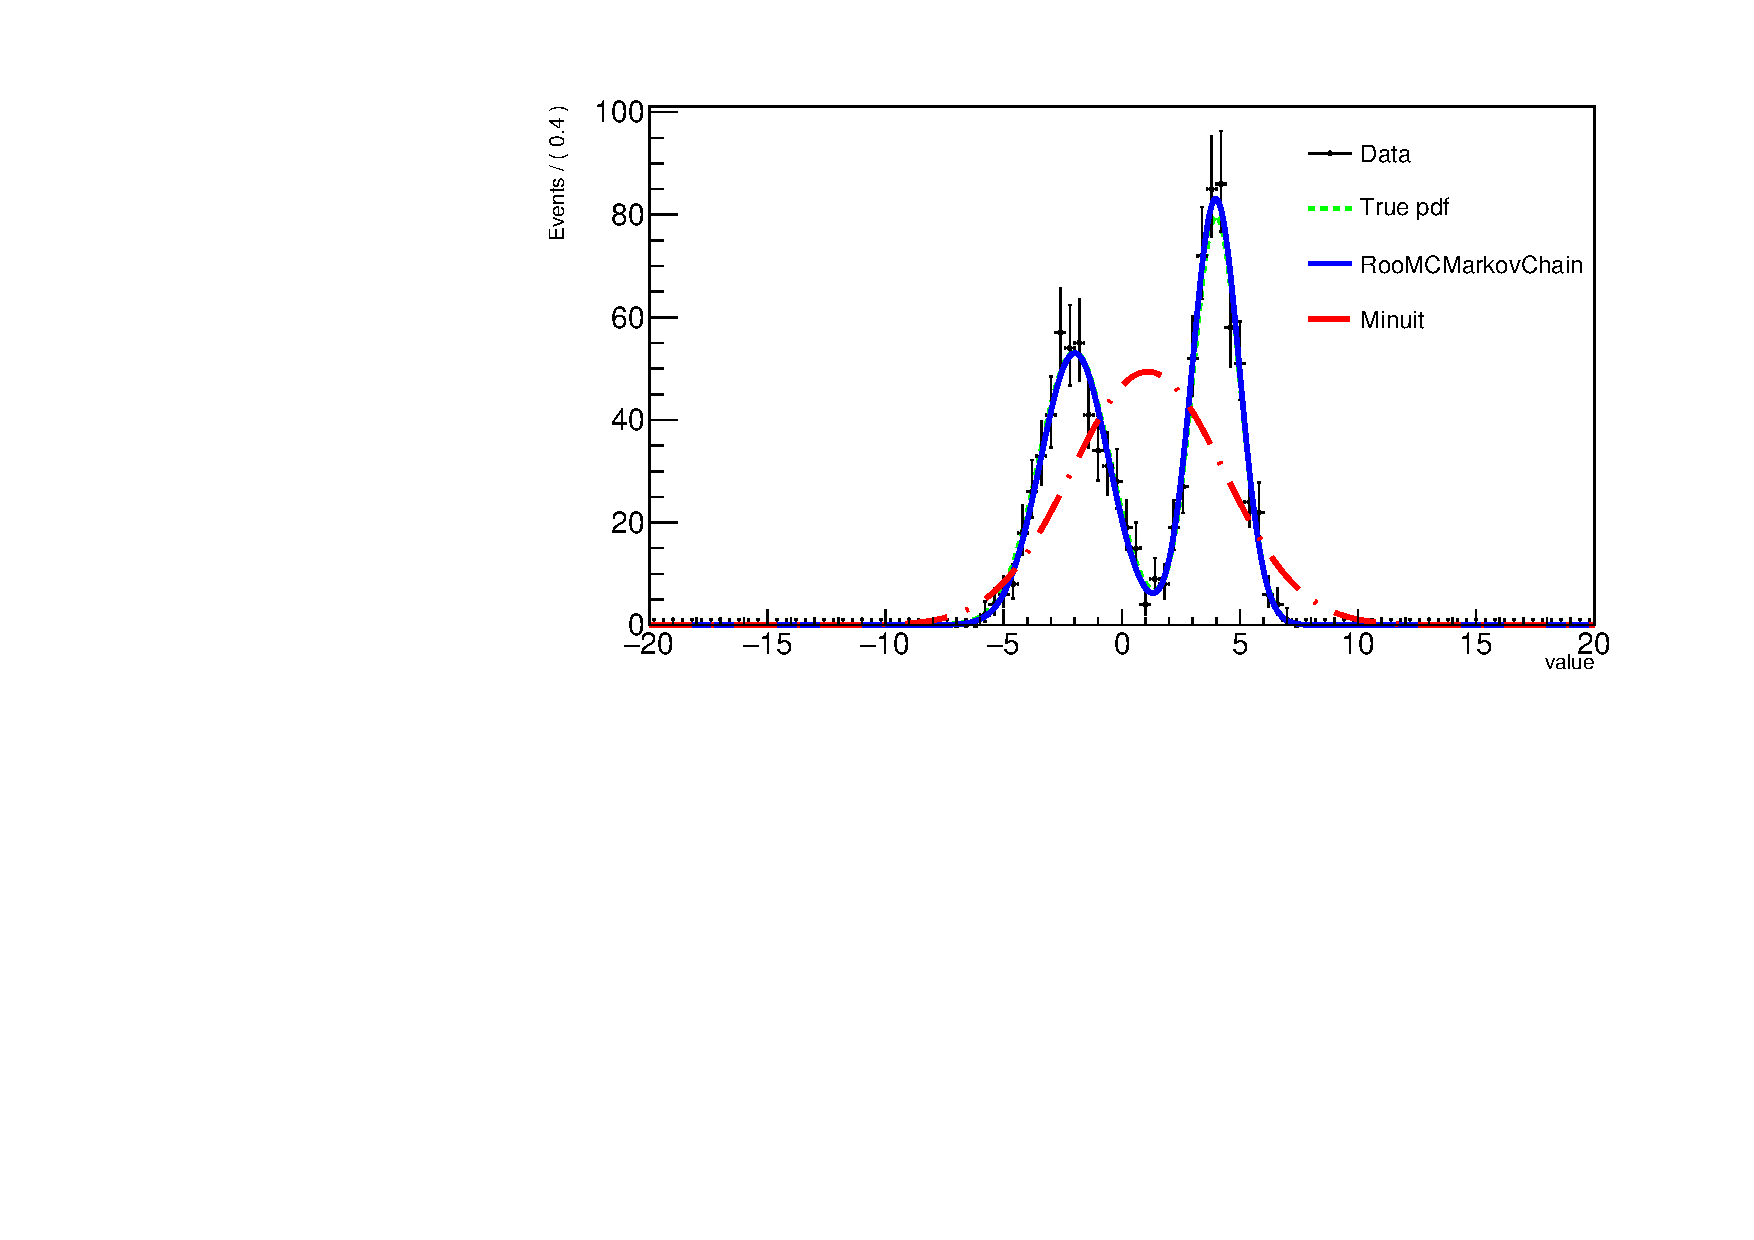
\includegraphics[width=0.8\textwidth]{RooMCMC/twogausfit}
  \caption{Fit of double gaus pdf (see equation \ref{eq:gausspdf}) with RooMCMCarkovchain and with Minuit. The true pdf has the follwing values: $\mu_1 = -2$, $\sigma_1 = 1.5$, $\mu_2 = 4$, $\sigma_2 = 1$ and the fraction $f = 0.5$. The Minuit fit fails, because of a unknown error. The fits gets right if the starting values for the parameters are changed.}
  \label{fig:twogaus}
\end{figure}
Figure \ref{fig:twogaus} shows that the Minuit routine fails to fit the distribution. The reasons are unknwon, but the fit gets right if the starting values of the parameters are changed. Intensive testing prooved RooMCMarkovChain less sensitive to starting values. But one should analysis with the number of parameters usually used in particle physics, with up to 50 parameters. \\
The terminal output, for the fit in figure \ref{fig:twogaus}, gives the estimated parameters with error interval and correlation coefficents of each parameter pair.

\begin{figure}[H]
  \centering
  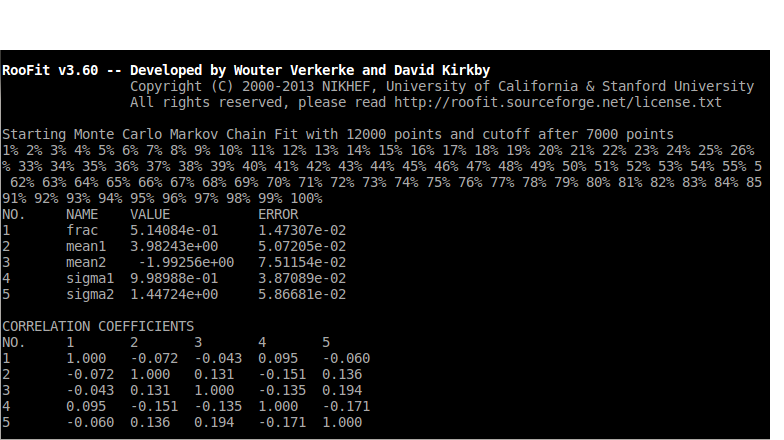
\includegraphics[width=0.8\textwidth]{RooMCMC/terminal_output}
  \caption{Terminal output of the RooMCMarkovChain fit. Note that RooMCMarkovChain confused the two means, because for the algorithm the two pdfs are equal.}
  \label{fig:terminal}
\end{figure}
This gives a good initial overview of results after the fit has finished. The error calculation can be set to assume gaussian or non-gaussian errors.

In addition several other properties of the parameters can be obtainded:
\begin{enumerate}
  \item The 1 dimensional profile of the negative log likelihood function for a given parameter.
  \begin{figure}[H]
    \centering
    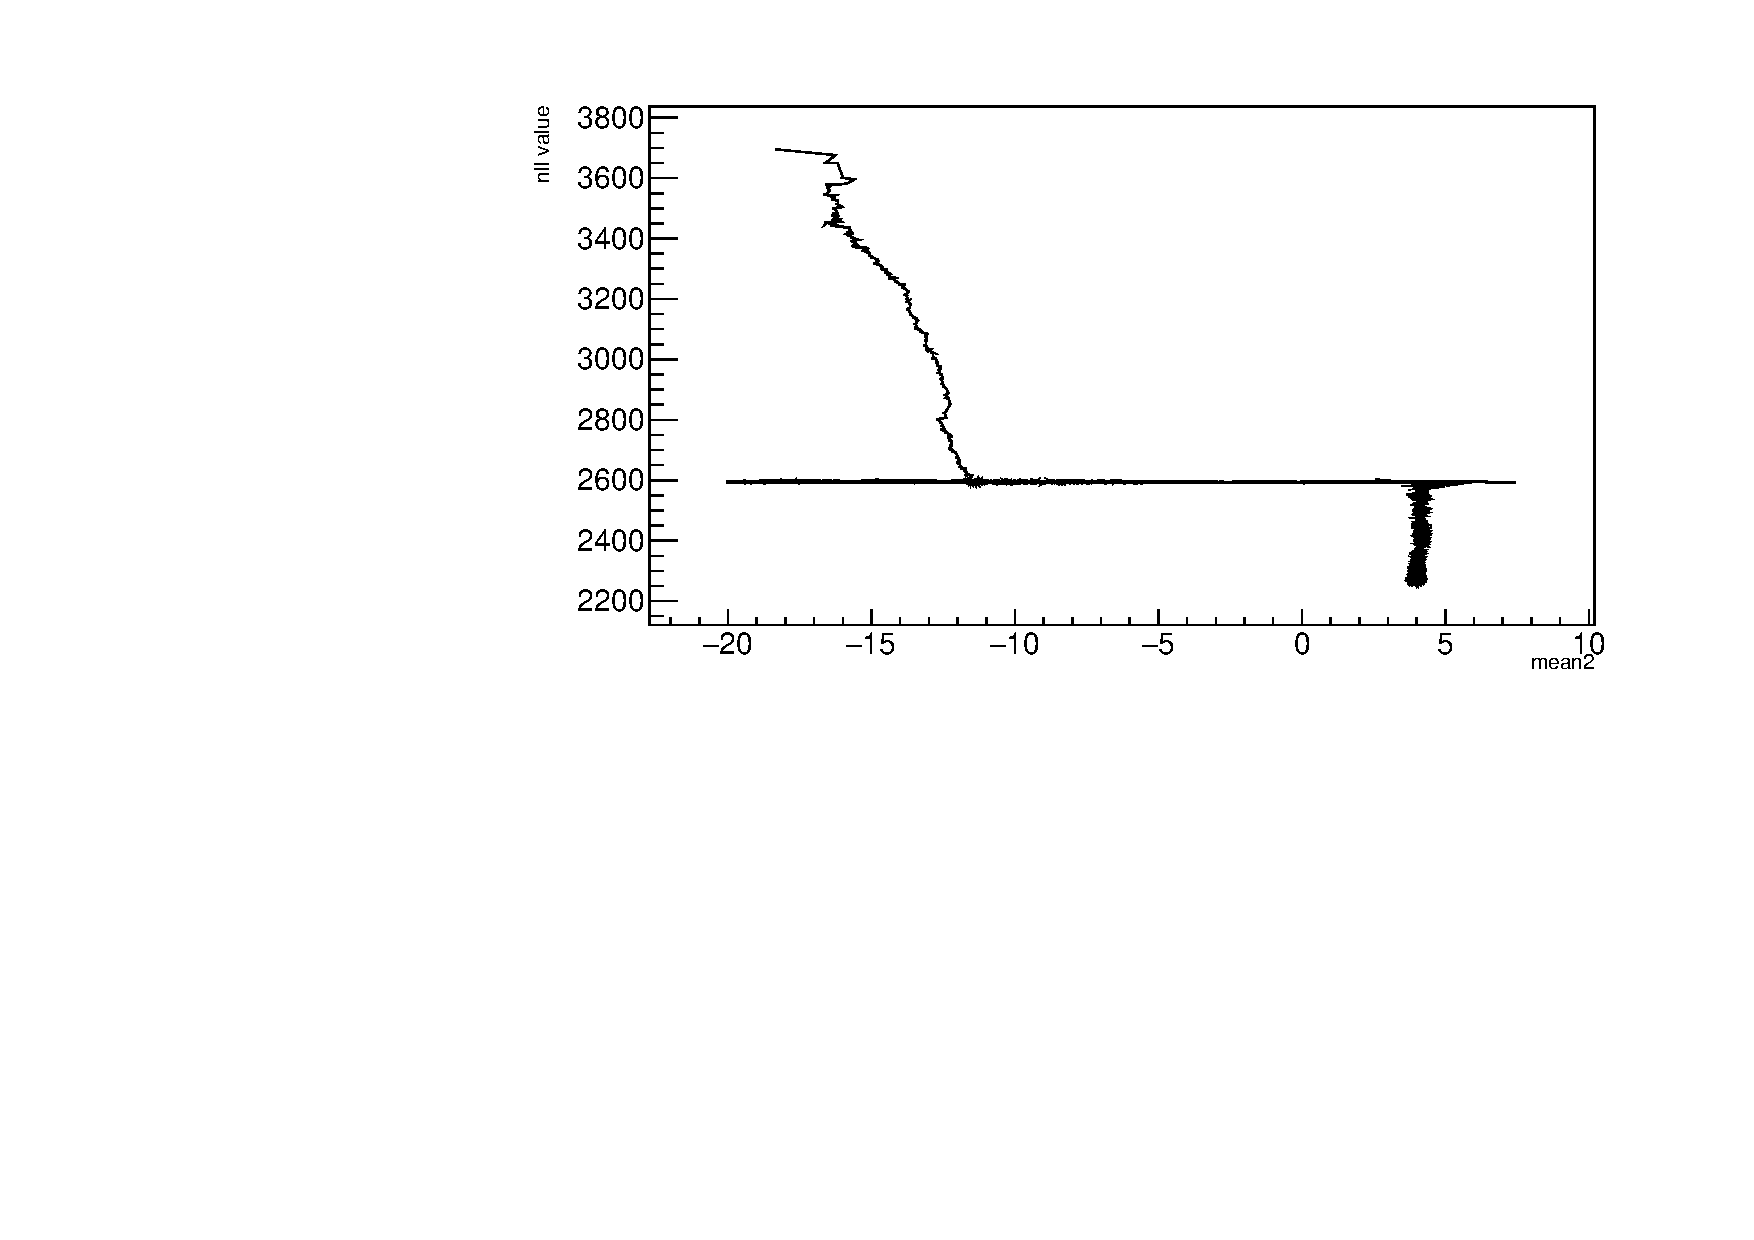
\includegraphics[width=0.8\textwidth]{RooMCMC/walkProfile}
    \caption{Profile of the negative log likelihood function for $\mu_2 = mean2$ in equation \ref{eq:gausspdf}. There is a local minimum at the nll value of 2600, since the algorithm scanned that region very briefly.}
    \label{fig:profile}
  \end{figure}
  From this plot on can see how the algorithm reached the minimum of the negative log likelihood function and if there are local minima. \\


  \item The walk distribution of a given parameter.
  \begin{figure}[H]
    \centering
    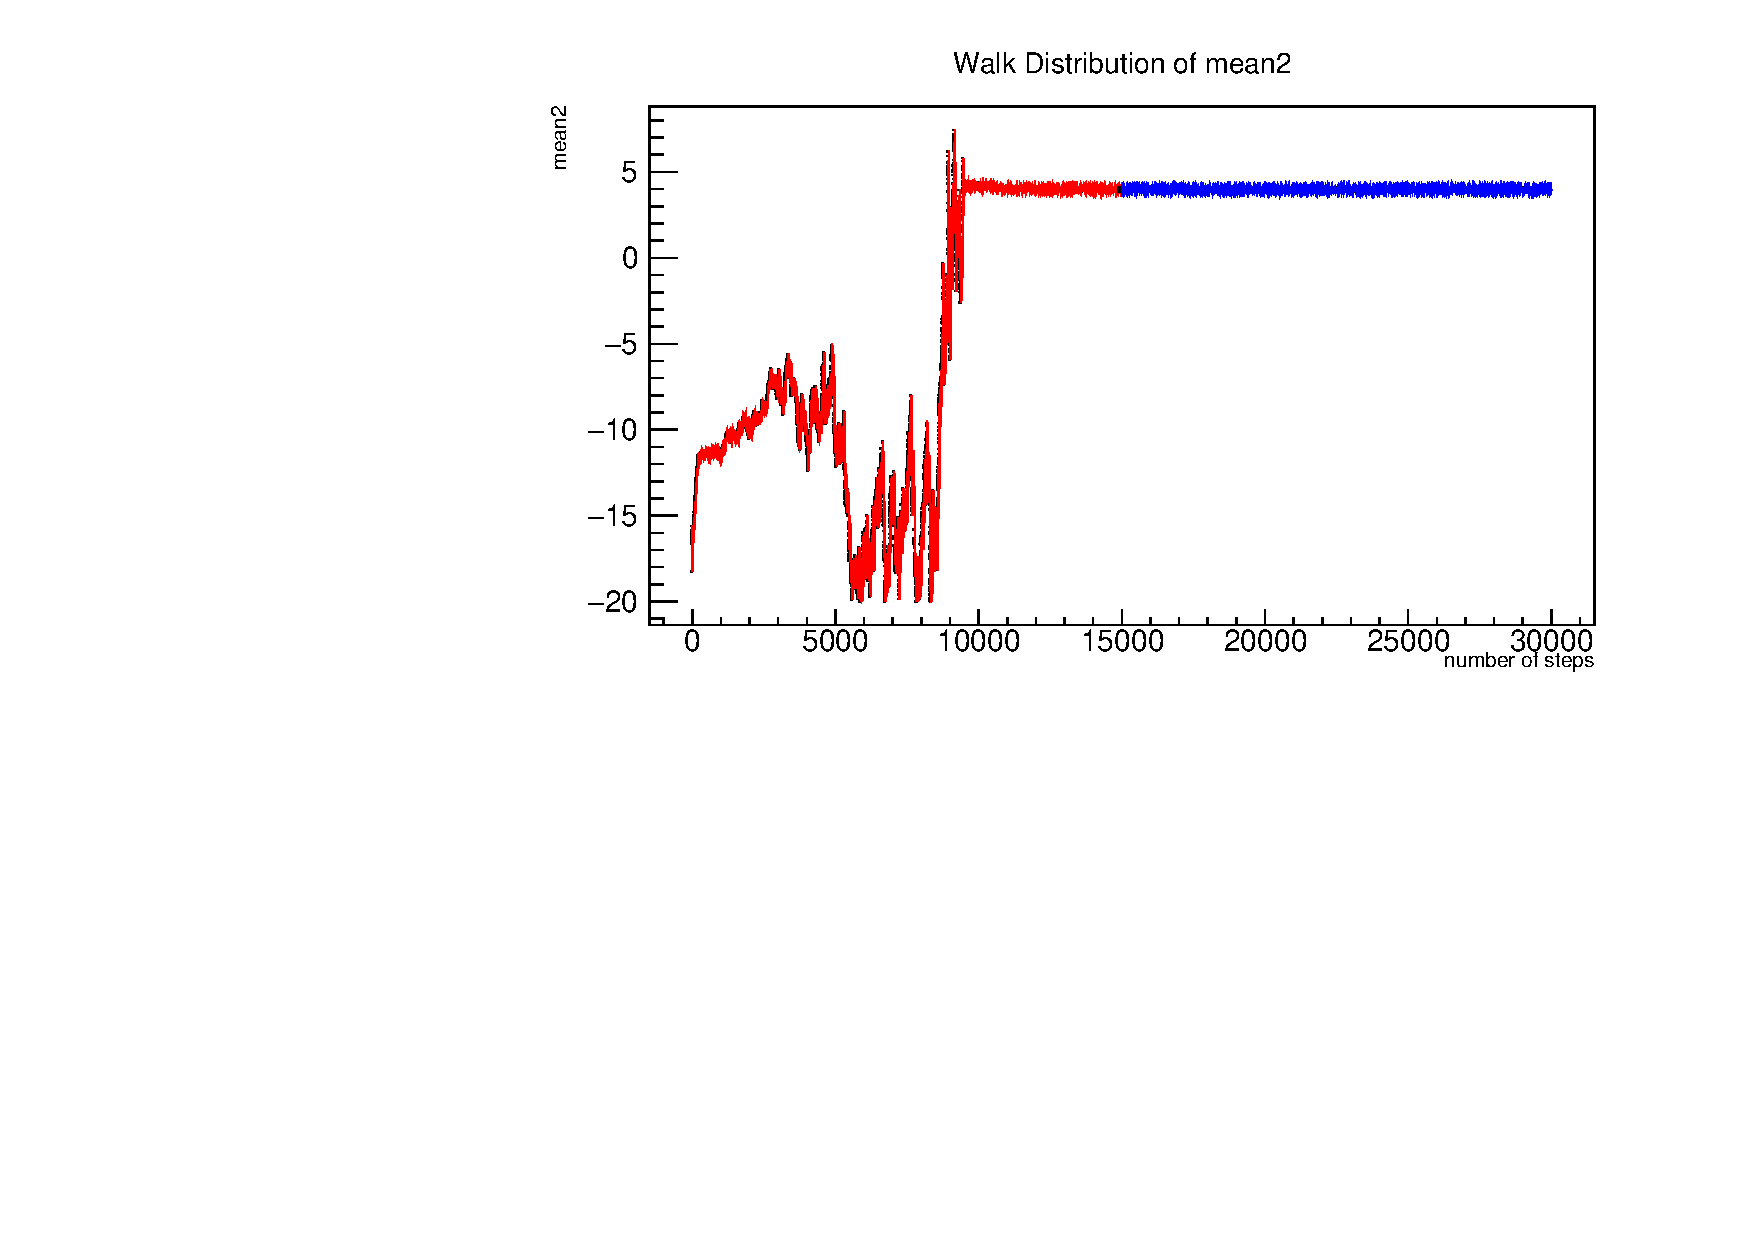
\includegraphics[width=0.8\textwidth]{RooMCMC/walkDis}
    \caption{Walk distribution of $\mu_2 = mean2$ in equation \ref{eq:gausspdf}. The red points are not considered for the error calculation, the number of points beeing cut of is defined by the user.}
    \label{fig:walkDis}
  \end{figure}
  This plot is very important for handling the RooMCMarkovChain class. Since the error calculation is based on the variance of the walk distribution, cutting of points in the begginning greatly reduces this variance. The user has to choose how many points are cut off. Plotting the walk distribution of all parameters helps choosing the right amount. The right amount would be at the point where there is only the oszillation arround the global minimum left. This has to be done by the user since there is now way to predict how many steps RooMCMarkovChain needs to reach the global minimum. \\

  \item The walk distribution of a given parameter as a histogramm.
  \begin{figure}[H]
    \centering
    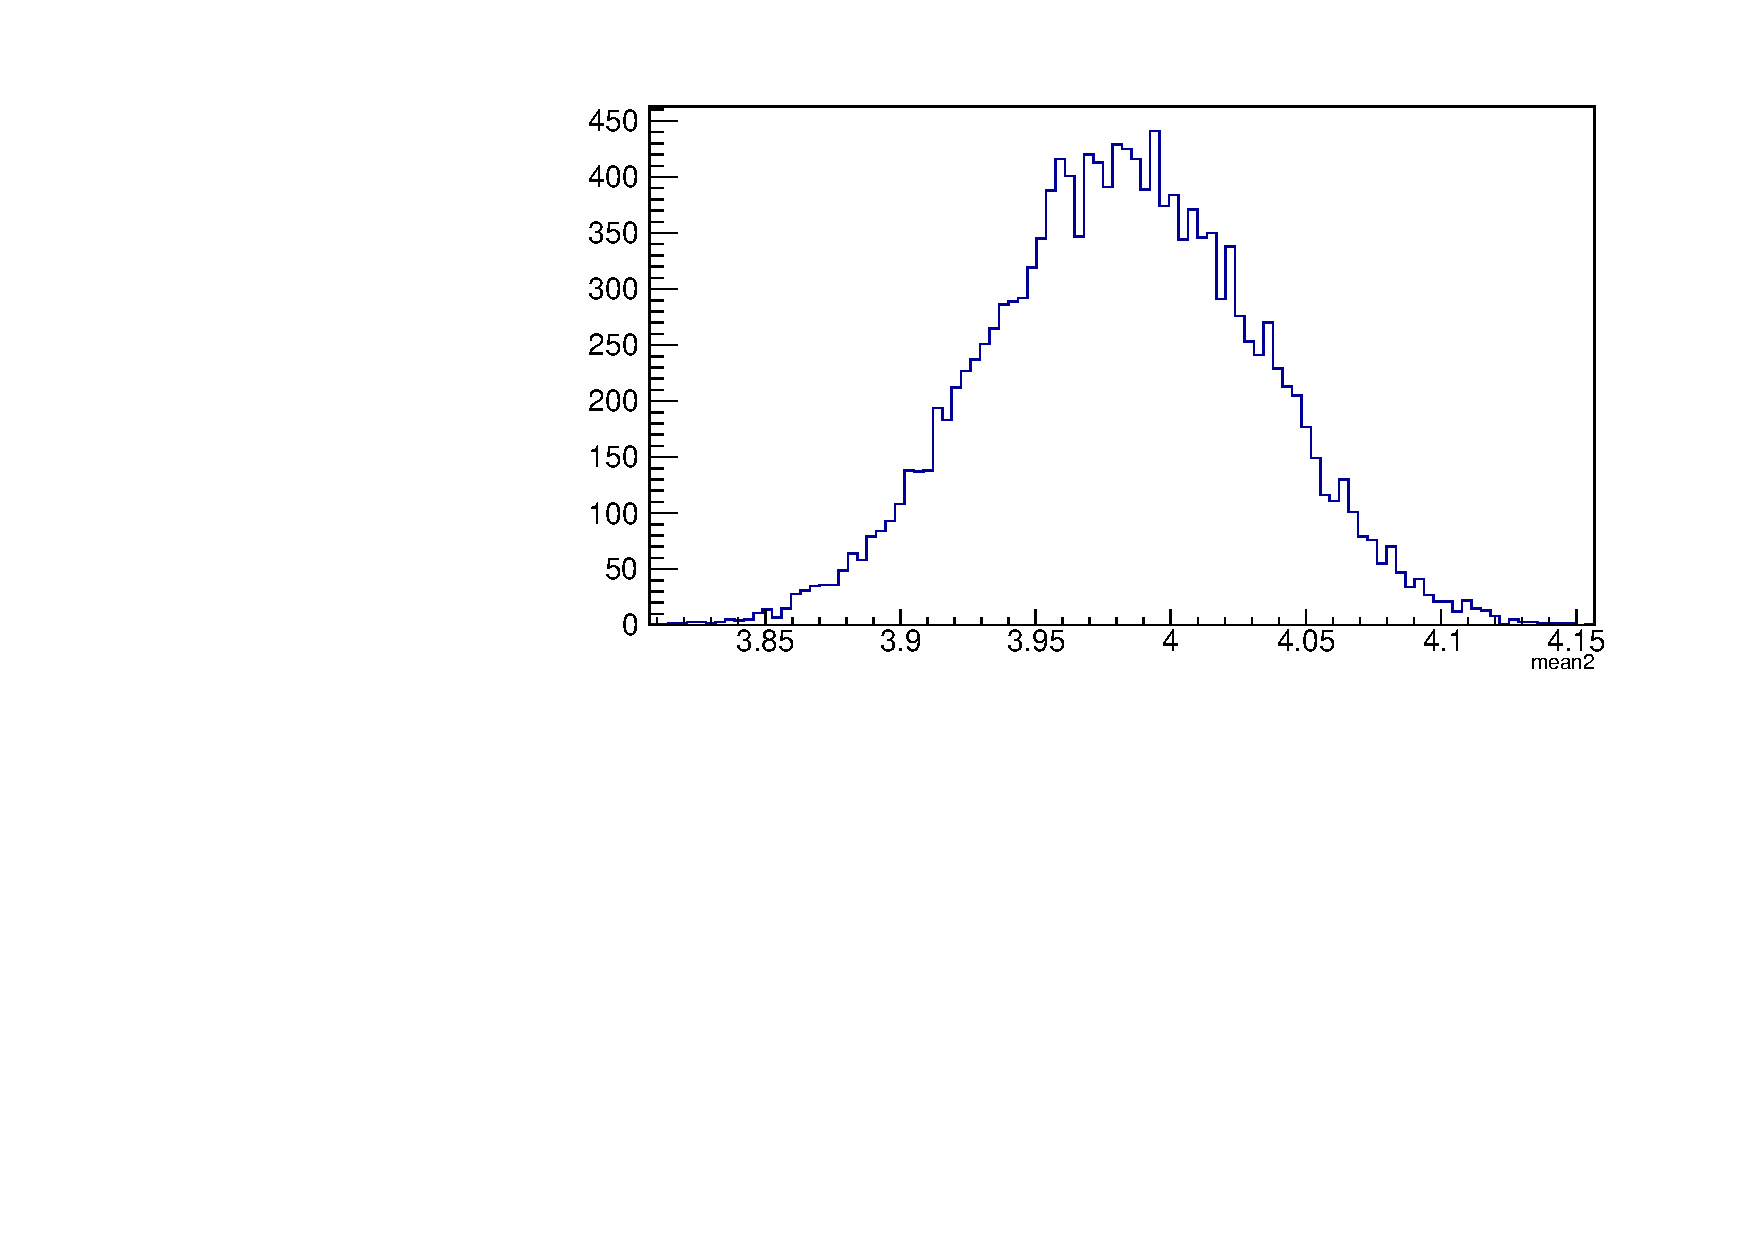
\includegraphics[width=0.8\textwidth]{RooMCMC/walkDisHis}
    \caption{Walk distribution of $\mu_2 = mean2$ in equation \ref{eq:gausspdf} as a histogramm.}
    \label{fig:walkDisHis}
  \end{figure}
  This plot can be used to check, which error strategy should be used. If the walk distribution histogramm is gaussian, gaussian errors can be assumed. \\

  \item The scatterplot between two given parameters.
  \begin{figure}[H]
    \centering
    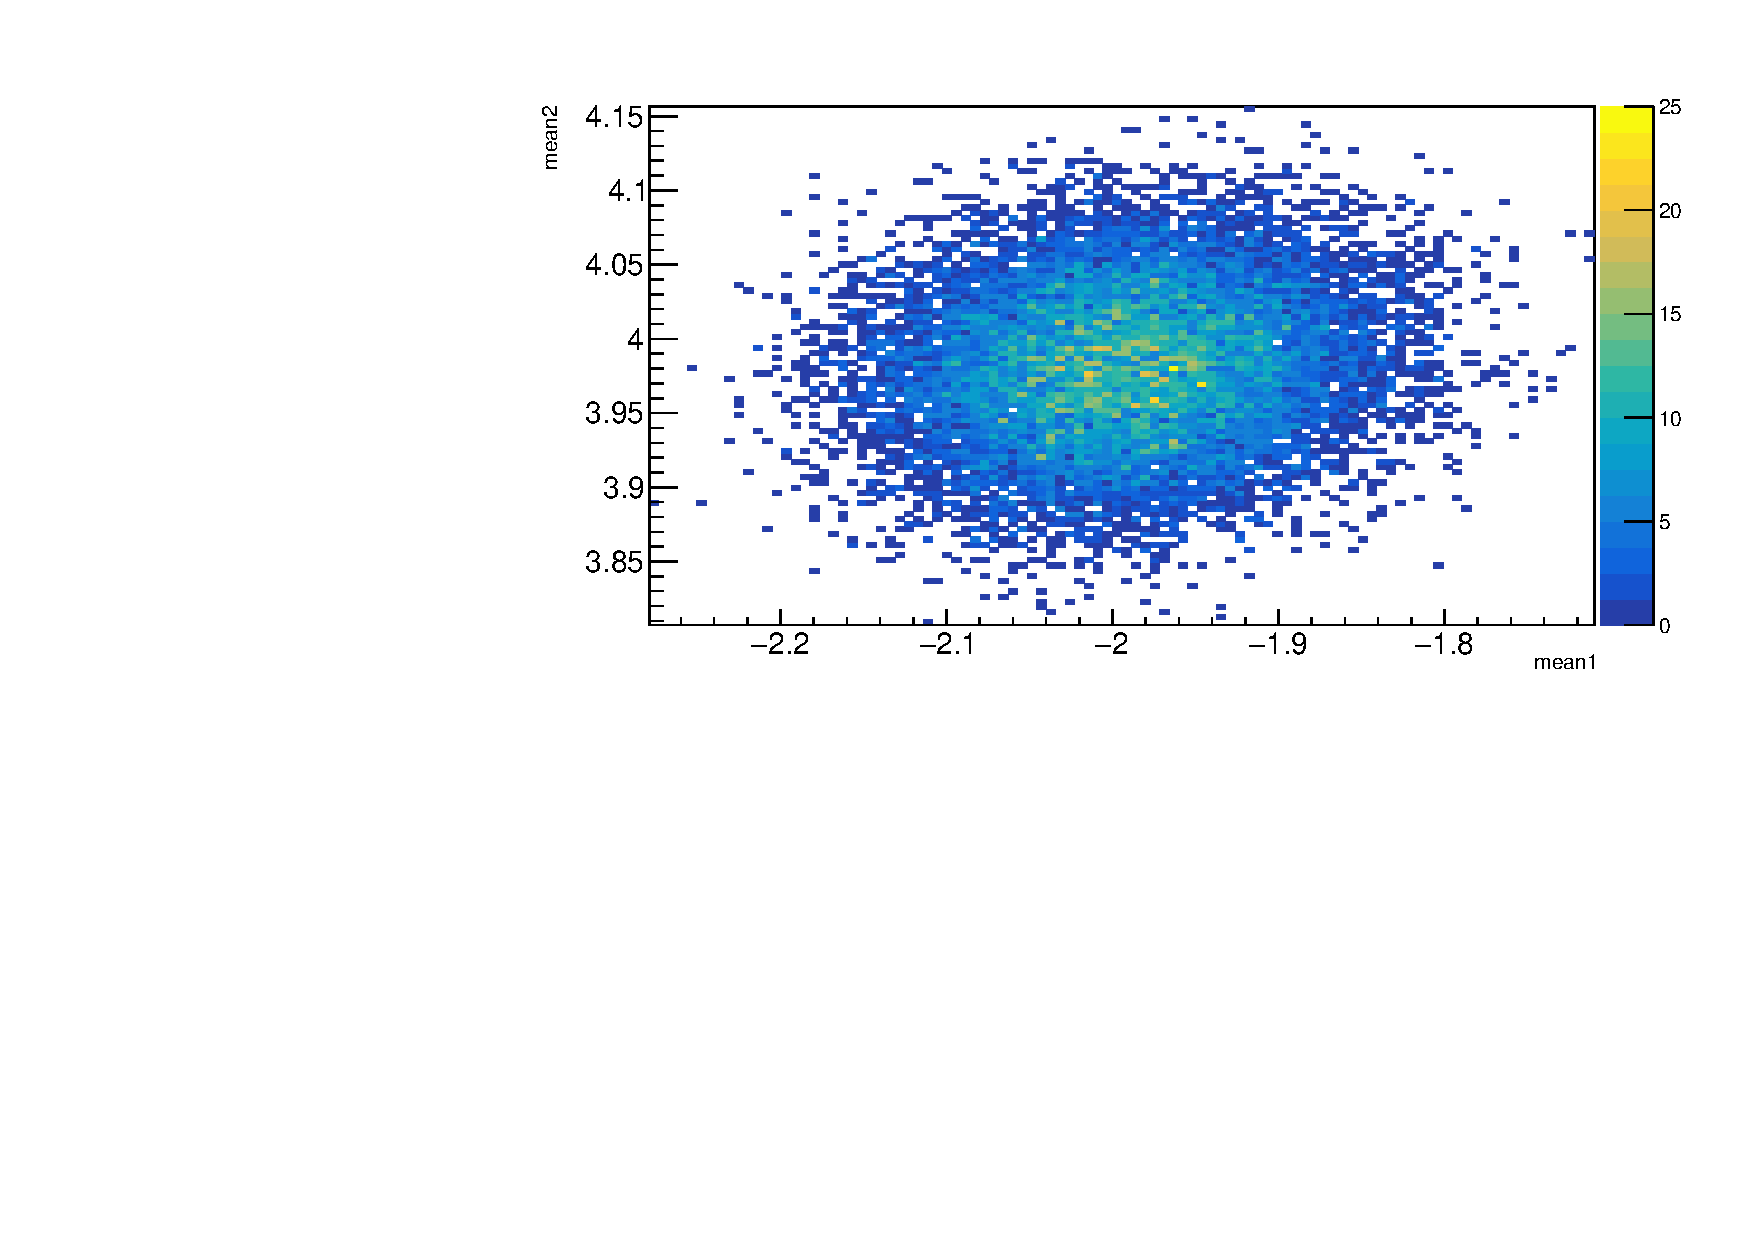
\includegraphics[width=0.8\textwidth]{RooMCMC/scatter}
    \caption{Scatterplot between $\mu_1$ and $\mu_2$ in equation \ref{eq:gausspdf}. The round shape states that there is no correlation between the two parameters.}
    \label{fig:scatter}
  \end{figure}
  This plot shows the correlation between two parameters graphically.
\end{enumerate}

%------------------------------------------------------------------------------

\section{Analysis of the $B$ $\rightarrow$ $K^{*}$ $\mu$ $\mu$ decay}

This section describes the motivation to analyse this decay, then the operators needed to calculate the different couplings are derived and in the last section the effetive Wilson coefficients are derived. This section is mostly theoretical and should give an overview over the decay.

\subsection{Motivation} \label{sec:Motivation}

In the Standart Model of particle physics the different leptons, Electron, Muon and Taoun only differ in there masses. Therfore if these leptons have a high energy (TeV) where the mass becomes negligible the leptons all behave the same. This phenomen is called lepton universality. For a long time it was one of the ground pillars of the Standart Model. But recent experimental results of the LHCb collaboration \cite{bib:LU} suggest a violation of the lepton universality. They measured the branching fraction of four $B$ deacys with a $b$ quark to $s$ quark transistion and two leptons in the final state. To reduce systematic uncertainties the following double ratio of these branching fractions has been considered a well defined test of lepton universaility. Since leptons at high energies should behave the same, this double ratio is expected to be equal to one.
\begin{equation}
  \begin{split}
  R_{K*0} &= \left. \dfrac{\mathcal{B}(B^0 \rightarrow K^{*0} \mu^+ \mu^-)}{\mathcal{B}(B^0 \rightarrow K^{*0} J/\psi(\rightarrow \mu^+ \mu^-))} \middle/   \dfrac{\mathcal{B}(B^0 \rightarrow K^{*0} e^+ e^-)}{\mathcal{B} ( B^0 \rightarrow K^{*0} J/\psi(\rightarrow e^+ e^-))}  \right. , \\
  R_{K*0} &=   \begin{cases}
    0.66^{+0.11}_{-0.07} (\text{stat}) \pm 0.03 (\text{syst}) \text{for} 0.045 < q^2 < 1.1 \text{ GeV}^2/c^4, \\
    0.69^{+0.11}_{-0.07} (\text{stat}) \pm 0.05 (\text{syst}) \text{for} 1.1 < q^2 < 6.0 \text{ GeV}^2/c^4.
\end{cases}
\end{split}
\end{equation}
The mesurement shows a 2.1-2.3 and 2.4-2.5 $\sigma$ deviation from the Standart Modell in the two $q^2$ regions, respectively.
To investigate further the same measurment is performed with new data from the LHCb detector. The goal of this thesis is to contribute to this new measuremnt.


\subsection{Kinematics} \label{sec:Kinematics}
In this section the decay itself and its kinematics are explained:
The Decay is a flavor changing neutral current (FCNC) with four charged particles in the final state. The FCNC is a current, which changes the flavor of a fermion without changing its electric charge. The four particles in the final stage are:  \\
The $K^+$ and $\pi^-$ from the $K^{*}$ decay and two leptons from the loop or box diagrams:
\begin{figure}[H]
 \centering
 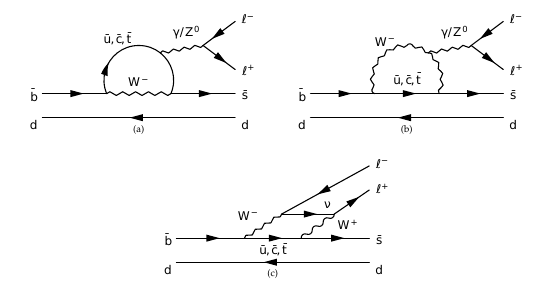
\includegraphics[width=0.8\linewidth]{KstarFeynman}
 \caption{Feynman diagrams for decay $B(\bar{b},d)$ $\rightarrow$ $ K^*(\bar{s},d) l^+$ $l^-$ at lowest order}
 \label{fig:Feynman}
\end{figure}
The kinematics of the decay are defined by the three angels $\theta_K$, $\theta_L$ and $\phi$, shown in figure \ref{fig:angels} and the invariant di-muon mass square $q^2$.
\begin{figure}[H]
 \centering
 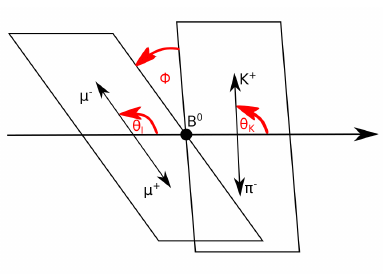
\includegraphics[width=0.6\linewidth]{angels}
 \caption{kinematic variables of the decay $B^0$ $\rightarrow$ $K^{*0}$ $\mu$ $\mu$}
 \label{fig:angels}
\end{figure}
The differential decay rate for the $B^0$ Meson can be expressed in terms of these variables:
\begin{equation}
 \begin{split}
  \frac{d^4 \Gamma}{d \cos{ \theta_L} d \cos{\theta_K} d \phi d q^2} &= \frac{9}{32 \pi} I(q^2,\theta_L, \theta_K, \phi) \\
  \text{with: } I(q^2,\theta_L, \theta_K, \phi) &= I_1^S \sin{^2(\theta_K)} + I_1^C \cos{^2 \theta_K} + \left(I_2^S \sin{^2 \theta_K} + I_2^C \cos{^2 \theta_K} \right) \cos{^2\theta_L} \\
  &+ I_3 \sin{^2 \theta_K} \sin{^2 \theta_L} \cos{2\phi} + I_4 \sin{2\theta_K} \sin{2\theta_L} \cos{\phi} \\
  &+ I_5 \sin{2\theta_K} \sin{ \theta_L} \cos{ \phi} \\
  &+ \left(I_6^S \sin{^2 \theta_K} + I_6^C \cos{^2 \theta_K}  \right) \cos{ \theta_L} + I_7 \sin{ 2\theta_K} \sin{\theta_L} \sin{\phi} \\
  &+ I_8 \sin{ 2\theta_K} \sin{ 2\theta_L} \sin{ \phi} + I_9 \sin{^2 \theta_K} \sin{^2 \theta_L} \sin{2 \phi}\\
 \end{split}
 \label{eq:diff_decay_rate}
\end{equation}
This decay rate is defined as the probability per unit time that the particle will decay. The $I_i$ can be obtained by fitting this decay rate to the kinematic variables obtained by the detector. This fit is usually done by a standart fitting routine called MINUIT \cite{bib:Minuit}. In section \ref{sec:RooMCMC} an alternative is presented. \\
For completness the next two sections desribe some of the theory concerning the decay: The operators and wilson coefficients.

\subsection{Operators for $B \rightarrow X_s l^+l^-$ decays}
In this section all the operators of the decay are derived from the effective Lagrangian. the operators in Quantum field theory are used to create or destroy particles, by applying them to a quantum field. This section should just give an overview if you need more detailed information consider reading reference \cite{bib:Operators}. \\
The effective Lagrangian for $B \rightarrow X_s l^+l^-$ decays has the form:
\begin{align}
 \mathcal{L}_{eff} & = \mathcal{L}_{QCD,QED}(u,d,s,c,b,e,\mu,\tau) \notag                                                                                           \\
                   & + \frac{4G_F}{\sqrt(2)} \left[ V_{us}^* V_{ub} (C_1^c P_1^u + C_2^c P_2^u) + V_{cs}^* V_{cb} (C_1^c P_1^c + C_2^c P_2^c) \right] \label{eq:La} \\
                   & + \frac{4G_F}{\sqrt(2)} \sum_{i=3}^{10} \left[ (V_{us}^* V_{ub} + V_{cs}^* V_{cb})C_i^c + V_{ts}^* V_{tb} C_i^t  \right]P_i . \notag
\end{align}
The first term in equation \ref{eq:La} contains the kinetic terms of the light SM particles as well as their QCD and QED interactions. The remaining two terms consist of $\Delta B = - \Delta S =1$ local operators of dimension $(d \leq 6)$, which contain those light fields. The mass of the s quark can be negleted in comparisson with the b mass. One gets the following operators:
\begin{equation}
 \begin{split}
  \mathcal{O}_1^u &= (\bar{s}_L \gamma_\mu T^a u_L)(\bar{u}_L \gamma^\mu T^a b_L),  \\
  \mathcal{O}_2^u &= (\bar{s}_L \gamma_\mu u_L) (\bar{u}_L \gamma^\mu b_L),  \\
  \mathcal{O}_1^c &= (\bar{s}_L \gamma_\mu T^a c_L) (\bar{c}_L \gamma^\mu T^a b_L), g \\
  \mathcal{O}_2^c &= (\bar{s}_L \gamma_\mu c_L) (\bar{c}_L \gamma^\mu b_L),  \\
  \mathcal{O}_3 &= (\bar{s}_L \gamma_\mu b_L) \sum_q (\bar{q} \gamma^\mu q),  \\
  \mathcal{O}_4 &= (\bar{s}_L \gamma_\mu T^a b_L) \sum_q (\bar{q} \gamma^\mu T^a q),  \\
  \mathcal{O}_5 &= (\bar{s}_L \gamma_{\mu_1} \gamma_{\mu_2} \gamma_{\mu_3} b_L ) \sum_q (\bar{q} \gamma^{\mu_1} \gamma^{\mu_1} \gamma^{\mu_1} q),
 \end{split}
 \begin{split}
  \mathcal{O}_6 &= (\bar{s}_L \gamma_{\mu_1} \gamma_{\mu_2} \gamma_{\mu_3} T^a b_L) \sum_q (\bar{q} \gamma^{\mu_1} \gamma^{\mu_1} \gamma^{\mu_1} T^a q), \\
  \mathcal{O}_7 &= \frac{e}{g^2} m_b (\bar{s}_L \sigma^{\mu \nu} b_R) F_{\mu \nu},g \\
  \mathcal{O}_8 &= \frac{1}{g} m_b (\bar{s}_L \sigma^{\mu \nu} T^a b_R) G_{\mu \nu}^a,  \\
  \mathcal{O}_9 &= \frac{e^2}{g^2} (\bar{s}_L \gamma_\mu b_L) \sum_l (\bar{l} \gamma^\mu l),  \\
  \mathcal{O}_{10} &= \frac{e^2}{g^2} (\bar{s}_L \gamma_\mu b_L) \sum_l (\bar{l} \gamma^\mu \gamma_5 l),
 \end{split}
 \label{eq:P}
\end{equation}
where $\sum_q$ and $\sum_l$ denote the sums over light quarks and all leptons, respectivly.




\subsection{Wilson coefficients}
In this section the Wilson coefficents are derived from the effective Hamiltonion of the deacy.
The effective Hamiltonian for $b \rightarrow s \mu^+ \mu^- $ transitions can be written as:

\begin{align}
 H_{eff} = - \frac{4 G_F}{\sqrt{2}} \left(\lambda_t H_{eff}^{(t)} + \lambda_u H_{eff}^{(u)} \right) \label{eq:H}
\end{align}
The $\lambda_i$ can be expressed with CKM combinations $\lambda_i = V_{ib}V_{is}^*$.
\begin{align}
 H_{eff}^{(t)} & = C_1 \mathcal{O}_1^c + C_2 \mathcal{O}_2^C + \sum_{i=3}^6 C_i \mathcal{O}_i + \sum_{i=7,8,9,10,P,S} (C_i \mathcal{O}_i + C_i' \mathcal{O}_i') \label{eq:H(t)} \\
 H_{eff}^{(u)} & = C_1 ( \mathcal{O}_1^C - \mathcal{O}_1^u) + C_2 (\mathcal{O}_2^C - \mathcal{O}_2^u). \label{eq:H(u)}
\end{align}

The contribution of $H_{eff}^{(u)}$ has a double Cabibbo supression and is therefore usually dropped. It is kept here since it is sensitive to complex phases of decay amplitudes. The operators $\mathcal{O}_{i \leq 6}$ are the same as for general $B \rightarrow X_s l^+l^-$ decays, see equation \ref{eq:P}.
The remaining ones are given by:

\begin{equation}
 \begin{split}
  \mathcal{O}_7 &= \frac{e}{g^2} m_b (\bar{s} \sigma_{\mu \nu} P_R b) F^{\mu \nu}, \\
  \mathcal{O}_8 &= \frac{1}{g} m_b (\bar{s} \sigma_{\mu \nu} T^a P_R b) G^{\mu \nu a}, \\
  \mathcal{O}_9 &= \frac{e^2}{g^2} (\bar{s} \sigma_\mu P_L b) (\bar{\mu} \gamma^\mu \mu), \\
  \mathcal{O}_{10} &= \frac{e^2}{g^2} (\bar{s} \gamma_mu P_L b) (\bar{\mu} \gamma^\mu \gamma_5 \mu), \\
  \mathcal{O}_S &= \frac{e^2}{16 \pi^2} m_b (\bar{s} P_R b) (\bar{\mu} \mu), \\
  \mathcal{O}_P &= \frac{e^2}{16 \pi^2} m_b (\bar{s} P_R b)( \bar{\mu} \gamma_5 \mu),
 \end{split}
 \begin{split}
  \mathcal{O}_7^\prime &= \frac{e}{g^2} m_b (\bar{s} \sigma_{\mu \nu} P_L b) F^{\mu \nu}, \\
  \mathcal{O}_8^\prime &= \frac{1}{g} m_b (\bar{s} \sigma_{\mu \nu} T^a P_L b) G^{\mu \nu a}, \\
  \mathcal{O}_9^\prime &= \frac{e^2}{g^2} (\bar{s} \gamma_\mu P_R b) (\bar{\mu} \gamma^\mu \mu), \\
  \mathcal{O}_{10}^\prime &= \frac{e^2}{g^2} (\bar{s} \gamma_\mu P_R b) (\bar{\mu} \gamma^\mu \gamma_5 \mu), \\
  \mathcal{O}_S^\prime &= \frac{e^2}{16 \pi^2} m_b (\bar{s} P_L b) (\bar{\mu} \mu), \\
  \mathcal{O}_P^\prime &= \frac{e^2}{16 \pi^2} m_b (\bar{s} P_L b) (\bar{\mu} \gamma_5 \mu),
 \end{split}
 \label{eq:P2}
\end{equation}
where $m_b$ denotes the running b mass in the $\overline{MS}$ scheme and g is the strong coupling constant and $P_{L,R} = ( 1 \pm \gamma_5)/2$. In the Standart Modell the primed Operators with opposite chirality to the unprimed operators vanish or are highly suppresd as are the $\mathcal{O}_S$ and $\mathcal{O}_P$. The contributions of $\mathcal{O}_{1,2,3,4,5,6}$ are neglected, since they are either heavily constrained or their impact turns out to be generically very small. For example in the left-right symmetric models or throughout gluino contributions in a general Minimal Supersymmetric Standard Model. \\
The $C_i$ coefficients in the equations \ref{eq:H(t)} and \ref{eq:H(u)} are called Wilson coefficients. They encode short-distance physics and New Physics effects. For the calculation a matching scale $\mu = m_W$ is chosen, in a pertubative expansion in powers of $\alpha_s (m_W)$. Then the Wilson coefficents are evolved down to scales $\mu = m_b$ according to the solutions of the renomalization group equations. Contributions by New Physics enter through $C_i(m_W)$, while the low scales are determined by the Standart Modell. To allow a more organized expansion of the Wilson coefficients in pertubation theory the factors $16 \pi^2 / g^2 = 4 \pi / \alpha_S$ are included into the definitions of the operators $\mathcal{O}_{i \geq 7}$. All the $C_i$ expand as:
\begin{align}
 C_i = C_i^{(0)} + \frac{\alpha_s}{4 \pi} C_i^{(1)} + \left( \frac{\alpha_s}{4 \pi} \right)^2 C_i^{(2)} + O(\alpha_s^3)
\end{align}
where $C_i^{(0)}$ is the tree-level contribution, which is quale to zero for all operators except $\mathcal{O}_2$ and $C_i^{(n)}$ denotes the n-loop contributions.
Before discussing the Wilson coefficents in details, lets look at the Operators again; the operators $\mathcal{O}_S^\prime$ and $\mathcal{O}_P^\prime$ are given in terms of conserved currents. They carry no scale-dependence. They do not mix with other operators and their Wilson coefficents are at the matching scale. $\mathcal{O}_9$ is also given by conserved curents. It mixes with $\mathcal{O}_{1,2,3,4,5,6}$ via a virtual photon decaying into $\mu^+ \mu^-$. In addition their is a scale depedence from the factor $1/g^2$. This dependence is also present in $C_{10}$ which otherwise would be scale independent. \\
$C_7$ and $C_9$ always appear in a particular combination with other Wilson coefficents in matrix elements. Therfore effective coefficients are defined:
\begin{equation}
 \begin{split}
  C_7^{eff} &= \frac{4 \pi}{\alpha_s} C_7 - \frac{1}{3} C_3 - \frac{4}{9} C_4 - \frac{20}{3} C_5 - \frac{80}{9} C_6, \\
  C_8^{eff} &= \frac{4 \pi}{\alpha_s} C_8 + C_3 - \frac{1}{6} + 20 C_5 - \frac{10}{3} C_6 , \\
  C_9^{eff} &= \frac{4\pi}{\alpha_s} C_9 + \mathcal{Y}(q^2), \\
  C_{10}^{eff} &= \frac{4 \pi}{\alpha_s} C_{10}, \\
  C_{7,8,9,10}^{\prime eff} &= \frac{4 \pi}{\alpha_s} C_{7,8,9,10}^{\prime},
 \end{split}
\end{equation}
\begin{equation}
 \begin{split}
  \text{where   } \mathcal{Y} (q^2) &= h(q^2,m_c) \left( \frac{4}{3}C_1 + C_2 + 6C_3 + 60C_5 \right) \\
  &- \frac{1}{2} h(q^2,m_b) \left(7C_3 + \frac{4}{3}C_4 + 76C_5 + \frac{64}{3} C_6  \right) \\
  &- \frac{1}{2} h(q^2,0) \left( C_3 + \frac{4}{3}C_4 + 16C_5 + \frac{64}{3} C_6 \right) \\
  &+ \frac{4}{3} C_3 + \frac{64}{9} C_5 + \frac{64}{27} C_6 .
 \end{split}env
\end{equation}
The function $h(q^2,m_q)$ comes from the fermion loop and for completness is presented in equation \ref{eq:h(q2,m)} below. If you need more details consider reading reference \cite{bib:Wilson}.
\begin{align}
 h(q^2,m_q)                                            & = - \frac{4}{9} \left(\ln{\frac{m_q^2}{\mu^2}} - \frac{2}{3} - z \right) - \frac{4}{9}(2+z) \sqrt{|z-1|}  \cdot  \begin{cases}
 \arctan{\frac{1}{\sqrt{z-1}}}                         & z > 1                                                                                                                          \\
 \ln{\frac{1+ \sqrt{1-z}}{\sqrt{z}}} - \frac{i \pi}{2} & z \leq 1
 \end{cases}
 \label{eq:h(q2,m)} \\
 \notag z                                              & = \frac{4m_q^2}{q^2}
\end{align}


\subsection{The LHCb Experiment} \label{sec:LHCb}
In this section the experimental setup of the detector is presented, which recorded the data used in this thesis.
The Large Hadron Collider beauty experiment (LHCb) is one of four large experiments based at the CERN laboratory near Geneva in Switzerland. It is part of the Large Hadron Collider (LHC), a proton-proton accelerator and collider located in a vast unterground tunnel with 26.7 km circumference beneath the Swiss-French countryside.
The other three experiments are CMS and ATLAS which are dedicated to a wide range of physics and have therefore very large detectors. ALICE investigates quark-gluon plasma and therefore needs heavy ion collisions, instead of proton collisions. \\
The protons in the LHC have a kinetic energy of 7 TeV, which allows a collision energy, in the LHCb detector, of 13 TeV. In the year 2016 the LHCb had a recorded luminosity of $\SI{1906}{pb^{-1}}$. For this thesis 1'575'210 potential $B \rightarrow K^* \mu \mu$ events are used and refered as raw LHCb data.
LHCb is dedicated to falvour physics. It therefore investigates rare decays and CP violation in beauty and charm hadrons.

\begin{figure}[H]
 \centering
 \includegraphics[width=1.0\textwidth]{{{LHC_default}}}
 \caption{CERN's Accelerator Complex \cite{bib:lhc_img}: The protons get injected in the lineare accelerator LINAC2. Then they get pre-accelerated in 3 synchrotons (BOOSTER,PS,SPS) where the protons reach a kinetic energy of 450 GeV. That is the entering energy of the LHC which accelerates them futher up to 7 TeV, before they collide at the four detectors: CMS, ATLAS, LHCb and ALICE.}
 \label{fig:lhc}
\end{figure}



\subsubsection{The LHCb Detector}
The LHCb Detector has a fix target geometry, because beauty hadrons are manily produced at small angeles with respect to the beam pipe.

\begin{figure}[H]
 \centering
 \includegraphics[width=1.0\textwidth]{{{lhcb_detector}}}
 \caption{Basic layout of the LHCb detector \cite{bib:lhcb_detector}. The interaction point is inside the vertrex detector and the beam pipe passes through the center. The different subdetectors are the two Ring Imaging Cherenkov Detectors (RICH1 and RICH2), the tracking stations (TT and T1 to T3), the scintillator pad detector (SPD), the preshower electromagnetic calorimeter (ECAL), the hadronic calorimeter (HCAL) and the muon stations (M1-M5). }
 \label{fig:lhcb_detector}
\end{figure}


\textbf{VErtex LOcator (VELO) \cite{bib:velo} :} Velo picks out B mesons from the multitude of other particles produced. This is a complex task since B mesons have very short livetimes spent colse to the beam. The VELO's silicon detecor elements must be placed at a distance of just five milimetres to the interaction point. To prevent damage to the detector during beam injection and stabilization it is mechanically moved to a safe distance. Velo measures B mesons indirectly be detecting its decay particles, nevertheless it has a resolution of $\SI{10}{microns}$.\\
\textbf{Ring Imaging Cherenkov (RICH) detectors \cite{bib:rich} :} The RICH detectors meeasure the emission of Cherenkov radiation, which happens when a charged particle passes through a medium faster than light does. It is a similar effect like the sonic boom a aircraft produces by breaking the sound barrier. The shape of the light cone depends on the particle's velocity, enabling the detector to determine the speed of a charged particle.  \\
\textbf{Magnet \cite{bib:mag} :} The big magnet of the LHCb experiment weights 27 tonnes and is mounted inside a 1,450 tonne steel frame. This powerful magnet forces all charged particels to change there trajectory. By examining the curvature of the path one can calculate the momentum of the particle.  \\
\textbf{Trackers \cite{bib:trac} :} The LHCb's tracking system consists of a series of four large rectangular stations, each covering an area of $\SI{40}{m^2}$. While flying through this area charged particles will leave a trace, therefor one can estimate the trajectory of a particle. The trajectory is used to link the signals left in other detecor elements to the corresponding particle. In LHCb two different tracker technologies are used: The silicon tracker placed close to the beam pipe, uses silicon microstripes. If a charged particle passes such a stripe it collides with the silicon atoms, liverating electrons and creating an electric current, which is then recorded. The outer tracker situated further from the beam pipe consists of gas-filled tubes. The gas ionizes when a charged particle hits a gas molecules, producing electrons. These reach an anode wire situated in the centre of each tube. The position of the track is found by timing how long it takes electrons to reach it. \\
\textbf{Calorimeters \cite{bib:calo} :} Calorimeters stop particles as they pass through, measuring the amount of energy lost. In LHCb there are two different types: The elctromagnetic calorimeter responsible for light particles like electrons and photons and the hadronic calorimeter responsible for heavier particles containing quarks. Both have a sandwich-like structure, with alternating layers of metal and plastic plates. If a particles hits a metal plate it produces a shower of secondary particles. These will excite polystyrenne molecules in the plastic plates, which then emit ultraviolet light. The energy lost by the particle in the metal plate is proportional to the amount of UV light produced in the plastic plates. \\
\textbf{Muon System \cite{bib:muonSys} :} The muon system consistes of 5 rectangular stations, which cover an area of $\SI{435}{m^2}$. Each station has chambers filled with three gases: carbon dioxide, argon and tetrafluoromethane. Passing muons react with the gas mixture and electrodes detect the result.


\subsubsection{The LHCb trigger system}
The rate of events at the LHCb interaction point is $\SI{40}{MHz}$. But the rate to have a B meson contained in the detector is $\SI{15}{kHz}$. The offline computing power just allows $\SI{2}{kHz}$ to be recorded. The LHCb trigger system aims to 'fill' this $\SI{2}{kHz}$ with intresting B decays and important control decays like $J/ \psi$ decays \cite{bib:JPsi}. The trigger has two levels: \\
The \textbf{Level Zero (L0)} trigger reduces the beginning $\SI{40}{MHz}$ to $\SI{1}{MHz}$. To get this high rate it can only rely on fast sub-detectors as the calorimeters and the muon system. The L0 trigger looks for events with high transverse momentum with respect to the patrticle beam axis (pT), because particles from a B decay have this attribute, since B Mesons are always produced almost parallel to the beam axis.
In addition the L0 trigger performs a simplified vertex reconstruction with the signal of two silicon layers of the VELO to identifie events with multple proton-proton collisions. They are rejected because for this kind of events its much more difiicult to reconstruct B meson decays, since it is harder to distinguish primary and secondary vertex of the B decay. \\
The \textbf{High Level Trigger (HTL)} is an algorithm that runs on a farm of 1000 16-core computers. It has two stages: HLT1 which reduces the event rate to a few tens of kHz and HLT2 which reduces the rate to the $\SI{2}{kHz}$ which are recorded. HLT1 gets all the candidates of the L0 trigger and uses the full detector information on them to search for particles with a high impact parameter with respect the proton-proton collision. These particles are most likly decay products from B mesons, because of its relatively long life-time. They typically fly 1 cm away from the collision before decaying resulting in a high impact parameter for the decay products. HLT2 does a complete reconstruction of the events. It starts with the track of the VELO and connects them to the tracks in the other sub-detectors. Most important are displaced vertices, since they are strong indicator for B decays. The selection is devided into two parts. The inclusive selection searches for resonance decays like $D^*$ or $J/ \psi$. The exclusive selection is desigened to provide the highest possible efficiency to fully reconstruct B decays of interest. It therfor uses all information available such as mass and vertex quality and intermediate resonances.






 % \subsection{Differential Decay Distribution}
 % In the experiments the observed decay is not $B \rightarrow K^* \mu \mu$, but $ B \rightarrow K^*(K \pi) \mu \mu$. This provides addition information on the polarization of the $K^*$ since the decay angle between $K$ and $\pi$ is senitiv to it. The matrix elemt of the effetive Hamiltonian (equation \ref{eq:H}) for this decay can be written as:
 % \begin{equation}
 %   \begin{split}
 %   \mathcal{M} &= \frac{G_F \alpha}{\sqrt{2} \pi} V_{tb} V_{ts}^* \Bigg \{ \bigg [ \braket{K \pi | \bar{s} \gamma^\mu ( C_9^{eff} P_L + C_9^{eff} P_R) b | \bar{B}}  \\
 %    &- \frac{2 m_b}{q^2} \braket{K \pi| \bar{s} i \sigma^{\mu \nu} q_\nu (C_7^{eff} P_L) b| \bar{b}} \bigg ] (\bar{\mu} \gamma_\mu \mu) \\
 %    &+ \braket{K \pi | \bar{s} \gamma^\mu ( C_{10}^{eff} P_L + C_{10}^{eff} P_R) b \bar{B}} (\bar{\mu} \gamma_5 \mu) \\
 %    &+ \braket{K \pi | \bar{s} (C_S P_R + C_S^\prime P_L) b|\bar{B}} (\bar{\mu} \mu) \\
 %    &+ \barket{K \pi | \bar{s} (C_P P_R + C_P^\prime P_L) b |\bar{B}} (\bar{\mu} \gamma_5 \mu) \Bigg \} .
 %  \end{split}
 %  \label{eq:M}
 % \end{equation}






 % \section{Contribution to the Analysis}
 %
 % This section presents the two contribution done for the analysis of the $B$ $\rightarrow$ $K^{*}$ $\mu$ $\mu$ decay. \\
 %  The first contributed to the eliminiation of combinatorial background. Combinatorial background is the background that is created due to the fact that in a hadron collider there are alwas several reaction happening at once. The different reaction combine to background.
 % To seperate the combinatorial background from the signal a classification is done. Classification is term from the Machine Learning field and means identifiying to which categorie an object belongs. For example consider having 100 pictures of animals and you want to know which ones are cats, dogs and cows. These are the categories and the pictures are the objects. The classification is perfomed by algorithms called classifieres. But before using them, they have to be trained. That is done by a training data set. It should look similar to the real data set, except that every object is labeld by its category. To get back to the animal pictures: One could create a training set by taking 5 pictures of a cat, 5 of a dog and 5 of a cow. These 15 pictures are the training set for the classifier. Now that the classifier knows how a cat, a dog and a cow looks like. It can identifie them in a random collection of pictures. \\

 % Ziel: Signal K* mu mu vom background zu trennen
 % combinatorial background erklaeren und entstehung

 \subsection{Selection} \label{sec:clas}

 \subsubsection{Inroduction to decision tree learning}

In particle physics the first step of each analysis is to clean up the data. That means to subtract the background from the signal. Signal means for example a type of decay like the $B \rightarrow K^* \mu \mu$ decay. To find this decay in the raw data of a detector which contains all kind of decays one needs thresholds on experimental parameters which are different or in the best case unique to the decay. That can be all kind of parameters like vertex locations, momentas or angles between trajectories. For the $B \rightarrow K^* \mu \mu$ decay these parameters would be:
\begin{itemize}
 \item Decay vertex location for reconstructed particles (ENDVERTEX)
 \item Primary vertex location (OWNPV)
 \item Impact parameter (IP\_OWNPV)
 \item Flight distance (FD\_OWNPV)
 \item The cosine of the angle between primary vertex and decay vertex and recorded momentum (DIRA\_OWNPV)
\end{itemize}
The names in the bracets are the labels given to these parameters in the data structure of the ROOT Data Anlysis Framework \cite{bib:root}.
Now one needs thresholds on these parameters, which define the signal-region. For example the flight distance has to be between 0.2 milimeters and 2 centimeters. But how do you obtain these thresholds? Thats were Classifiers are usefull. Classifiers are a type of algorithm from the Machine Learning area. They can be trained to distinguish different types of data. In this case signal and background. Each event in the data gets a probability to be signal assigend to it. So after the classification one can just take all the events with a probability over lets say 80\%. One has now eliminated 80\% of the background and can continue cleaning up the signal but thats not a part of this thesis. The goal of this part was to find the best classifier to be used in the  $B$ $\rightarrow$ $K^{*}$ $\mu$ $\mu$ decay analysis. \\
Seven different classifiers were tested. A test means that the classifier is given a training set consisting of Monte Carlo simulated events containing only $B$ $\rightarrow$ $K^{*}$ $\mu$ $\mu$ decays and randomly choosen real detector data, containing all kind of decays. In a training set the data is labeled. The Monte Carlo events are labeld with $1$ for signal and the real data with $0$ for background. The classifier will now train, that means the algorithm tries to label the data into signal and background by choosing different thresholds on the parameters mentioned above. After the training the thresholds get fixed. Now one has to test the classifer to check if everything worked fine. To do so a second set of data is prepared similar to the training set, just that the labels are now hidden from the classifier. Since the classifiers are not perfect, they do not assign $0$ and $1$ to each event but rather a probability to be signal between 0 and 1. A good classifier will now label the signal events with a high probability and background with a low probabillity. A bad classifier will assign 0.5 probability to each event.
With a 0.5 probability no information was gained by classification, because having a 50:50 chance is as good as guessing. This probability assignements can now be used as a threshold themselves to subtract the background. \\
Another property of classifiers is, that the data used in the training, can no longer be used in the analysis, because the classifier knows the training set too well and a bias is introduced if one reuses the training data in the actual analysis. That would mean that the part of the real detector data which is needed to train the classifiers would be lost for further analysis. To avoid such a waste of data a technique called k-folding is used. \\
K-folding means that the no training set is created. But the data Monte Carlo Mix with signal events labeled with 1 and background events labeled with 0 is split into k equal parts. Now to classify one part all the other parts are used for training, while the labels of the one part are of course hidden. After iterating over all parts, one has classified all the data without loosing any. The only disadvantage are the addidtional computer resources needed, since the classifier has now to be trained k times instead of one time.

 The following list of classifers where tested and compared in terms of perfomance:
 \begin{itemize}
  \item Ada Boost \cite{bib:AdaBoost}
  \item uGB \cite{bib:ugb} + knnAda (k-nearest neghbor AdaBoost)
  \item uBoost \cite{bib:uBoost}
  \item uGB \cite{bib:ugb} + Fl (flatness loss)
  \item xgb \cite{bib:xgb}
  \item sk\_bdtg \cite{bib:bdtg}
  \item sk\_bdt \cite{bib:bdt}
 \end{itemize}
 The test was performed with 30000 events from the 2016 LHCb $B$ $\rightarrow$ $K^{*}$ $\mu$ $\mu$ data and 10000 events from the Monte Carlo simulation.

To compare classifiers the so called ROC (receiver operating charactertic) curves are used. The ROC curve shows the true positive rate against the false positive rate. The true positive rate is the rate of signal events that have been classified correctly as signal events, while the false postive rate ist the rate of background events classified as signal events. On figure \ref{fig:roc} a ROC curves of the classifiers above is displayed.
The sample of 40000 events to test the classifiers was cut into ten equal parts, also called folds. In figure \ref{fig:roc} the ROC curve of one of these folds is displayed, the other nine can be found in the appendix \ref{app:roc}. \\
 It turns out that all the classifiers classify the data mostly correctly with just some minor variances. The ROC curve is in that case not a good tool to compare the different classifiers.
 \begin{figure}[H]
  \centering
  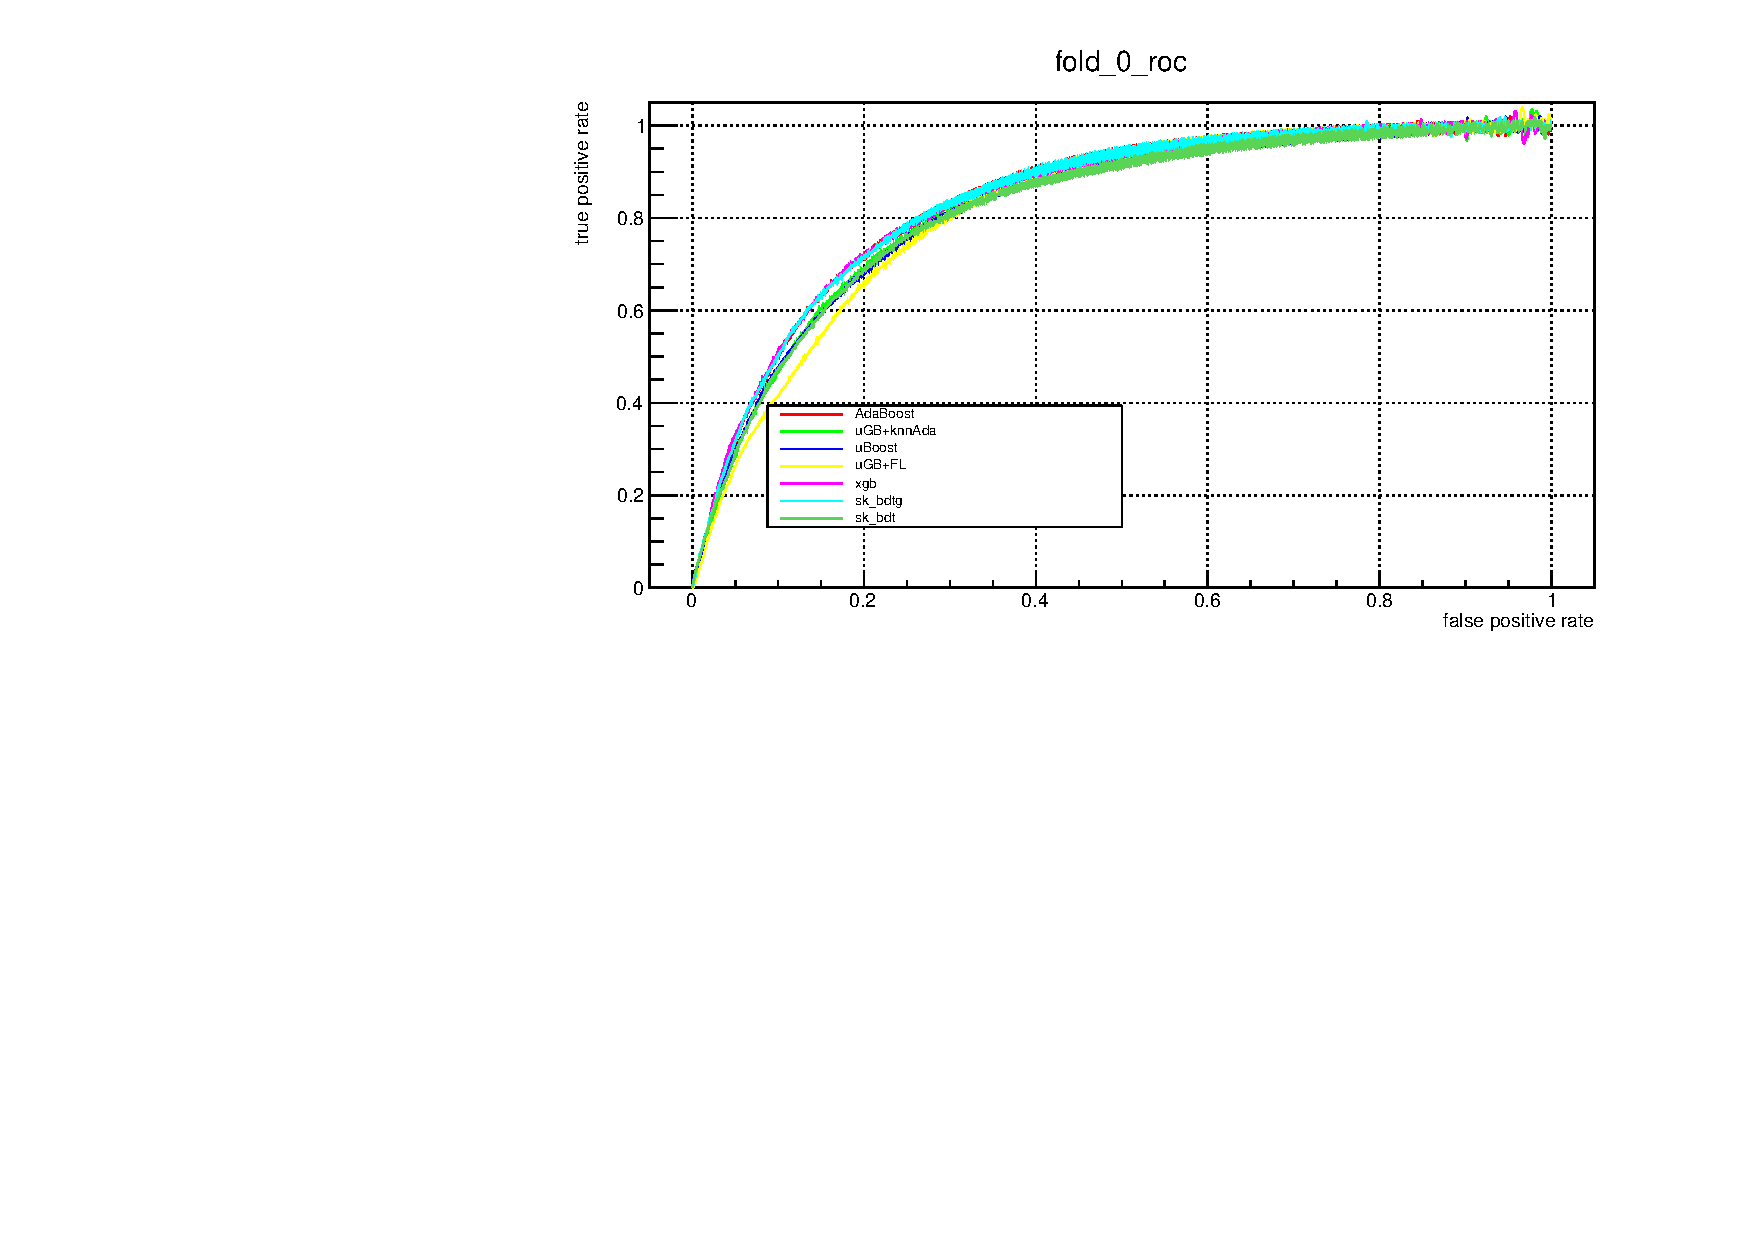
\includegraphics[width=0.8\textwidth]{roc/fold_0_roc.pdf}
  \caption{ROC curve of the first fold. One can see that all the classifiers are competetive in terms of classifing correctly}
  \label{fig:roc}
 \end{figure}
 The next step is to check for correlations between the assigned probabilities and the kinematic variables. The kinematic variabels as explained in section \ref{sec:Kinematics} are used to obtain the angular coefficients of the decay rate. If there is a correlation between the assigned probabilities from the classifier and these variables, a peak is artificialy added into the distribution of these variables. Imagine a positive correlation between the $B$ mass in the range 5000 to 6000 GeV and the probability to be signal from the classifier. After cutting at lets say 0.8 probability there will be a peak in the B mass distribution between 5000 and 6000 GeV. Normally such a peak suggest a new particle in this range. This is to avoid at all cost since it will compremise the whole analysis later on. \\
In the following the correlation between the probability to be signal assigned by the classifier and the $B$ mass are shown. The correlation plots for the other kinematic variables can be found in appendix \ref{app:corr}.


 % \begin{figure}[H]
 %  \centering
 %  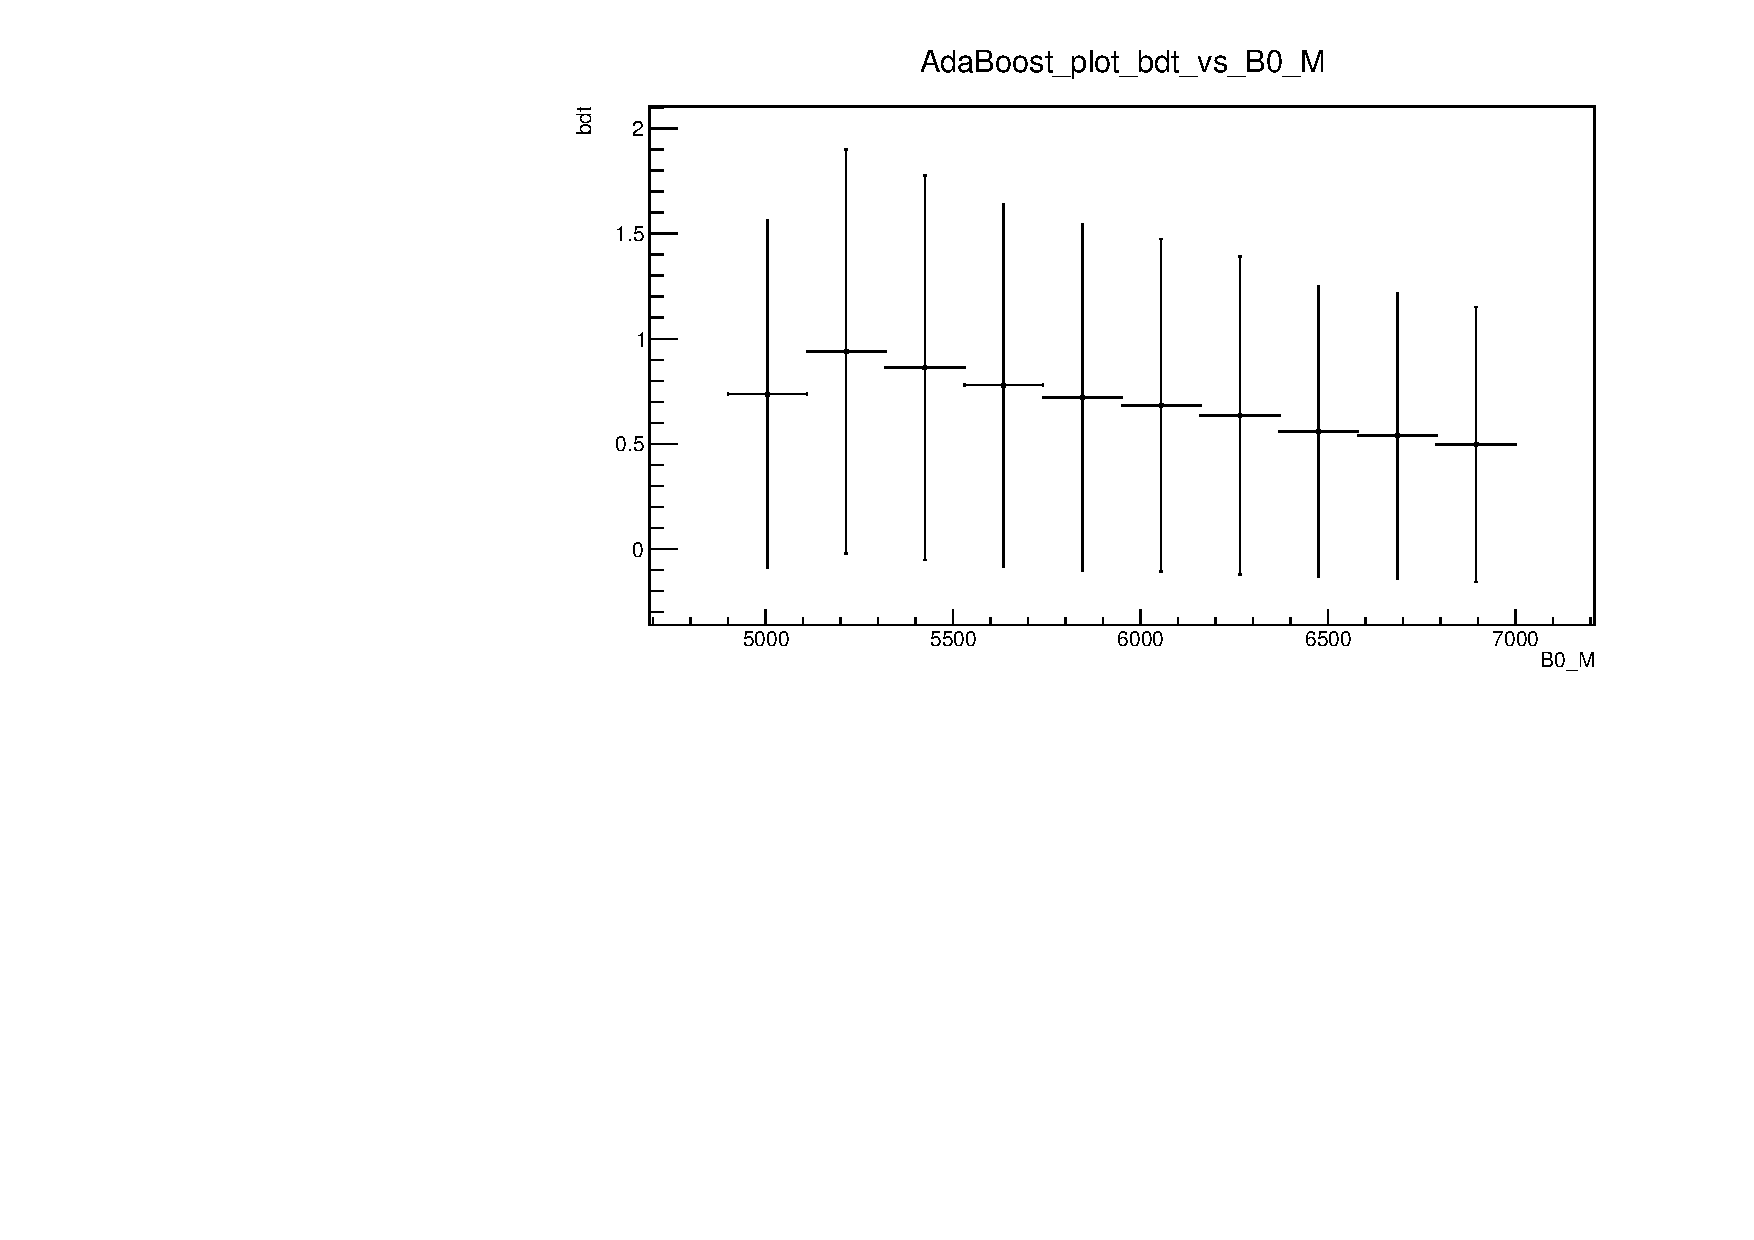
\includegraphics[width=0.5\textwidth]{plots/AdaBoost_plot_bdt_vs_B0_M}
 %  \caption{This plot shows the correltation between the bdt decision of the AdaBoost classifier and the $B$ mass. There is clearly a correlation starting from the second bin from the left.}
 %  \label{fig:AdaB0M}
 % \end{figure}

 \begin{figure}[H]
  \centering
  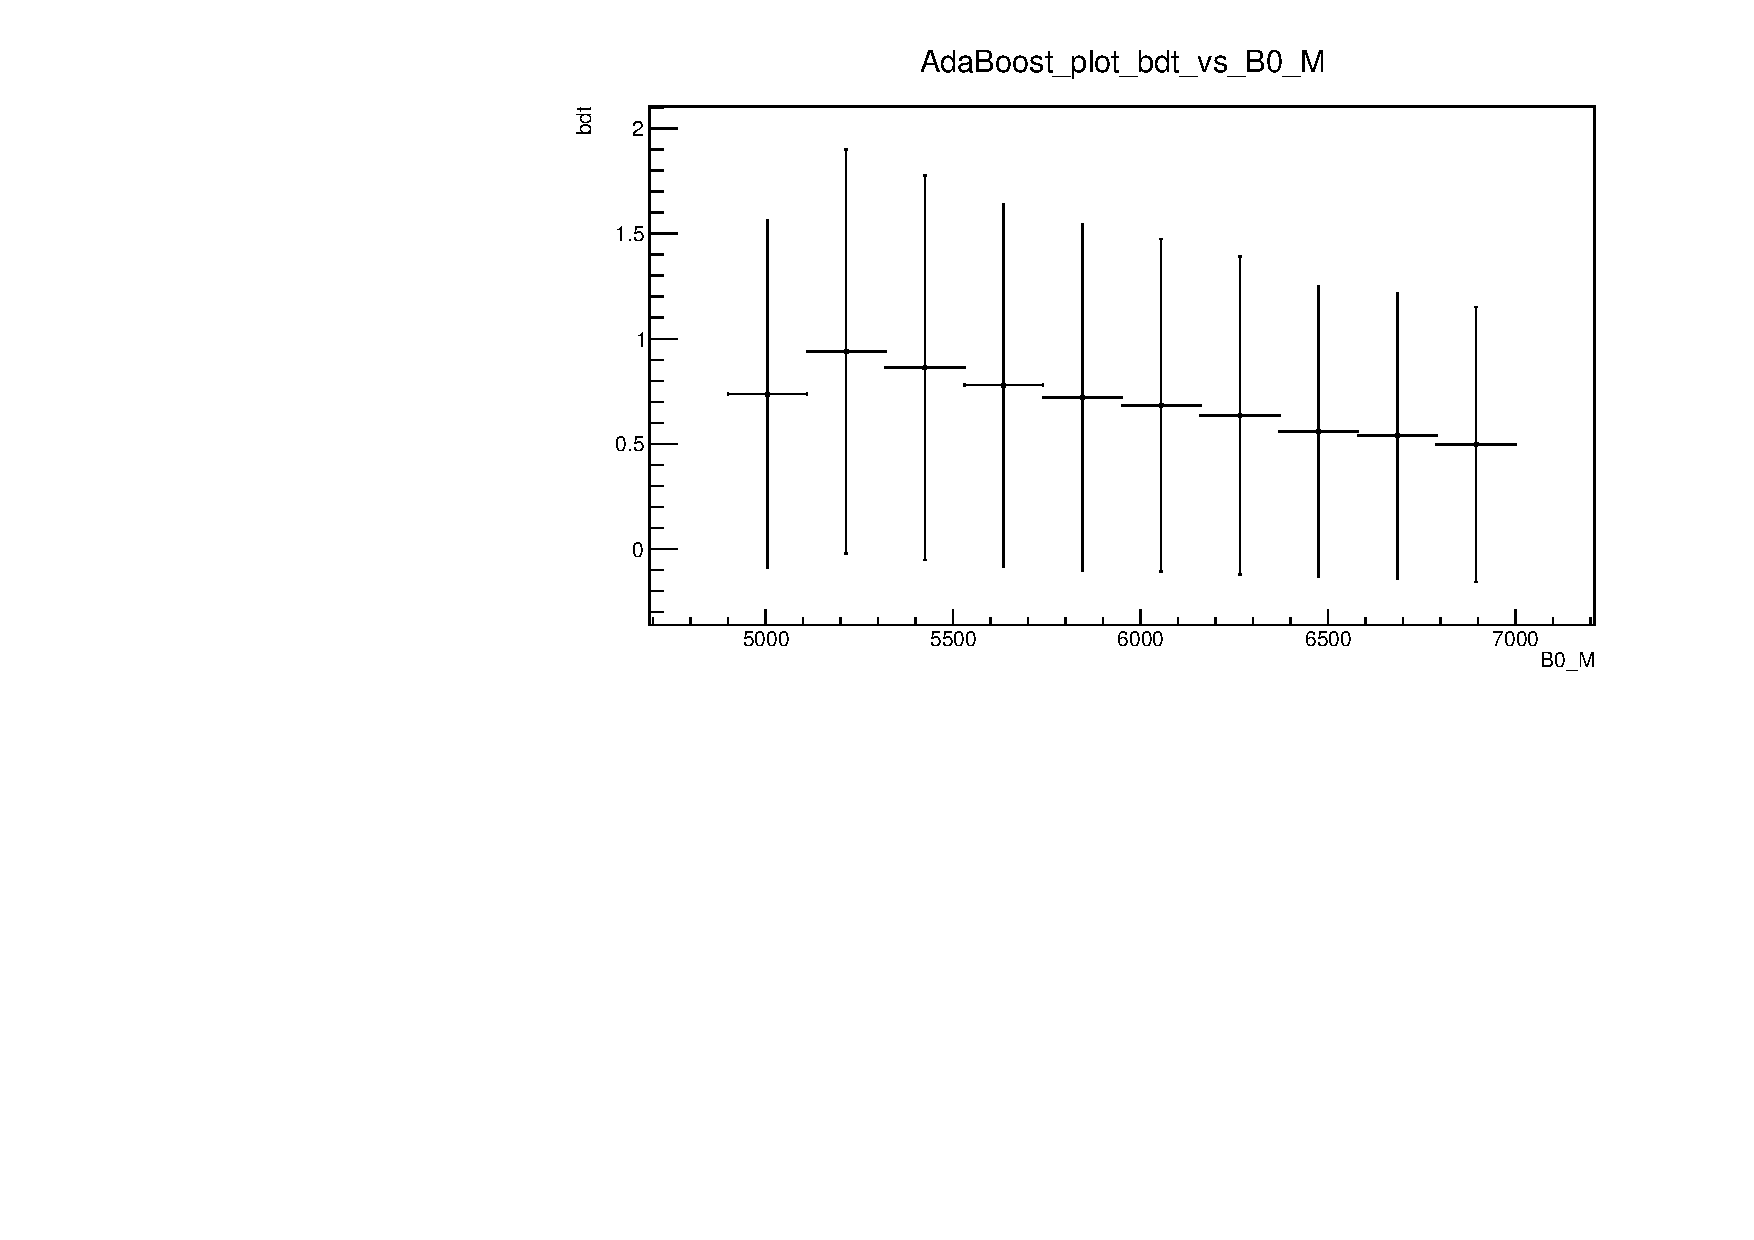
\includegraphics[width=0.5\textwidth]{plots/AdaBoost_plot_bdt_vs_B0_M}
  \caption{This plot showes the probabilities assign by the classifier as explained in the above paragraph, labeld with bdt on the Y achsis. On the X achsis the values for the $B$ mass are shown in MeV. The X - errorbars indicate the length of each bin, while the Y errorbars represent the standart derivation on the probabilities. One can see in this plot the correlation between the classifiers probabilities and the $B$ mass for the AdaBoost classifier. There is an obvius correlation from the second bin to the fourth bin.}
  \label{fig:AdaB0M}
 \end{figure}

 \begin{figure}[H]
  \centering
  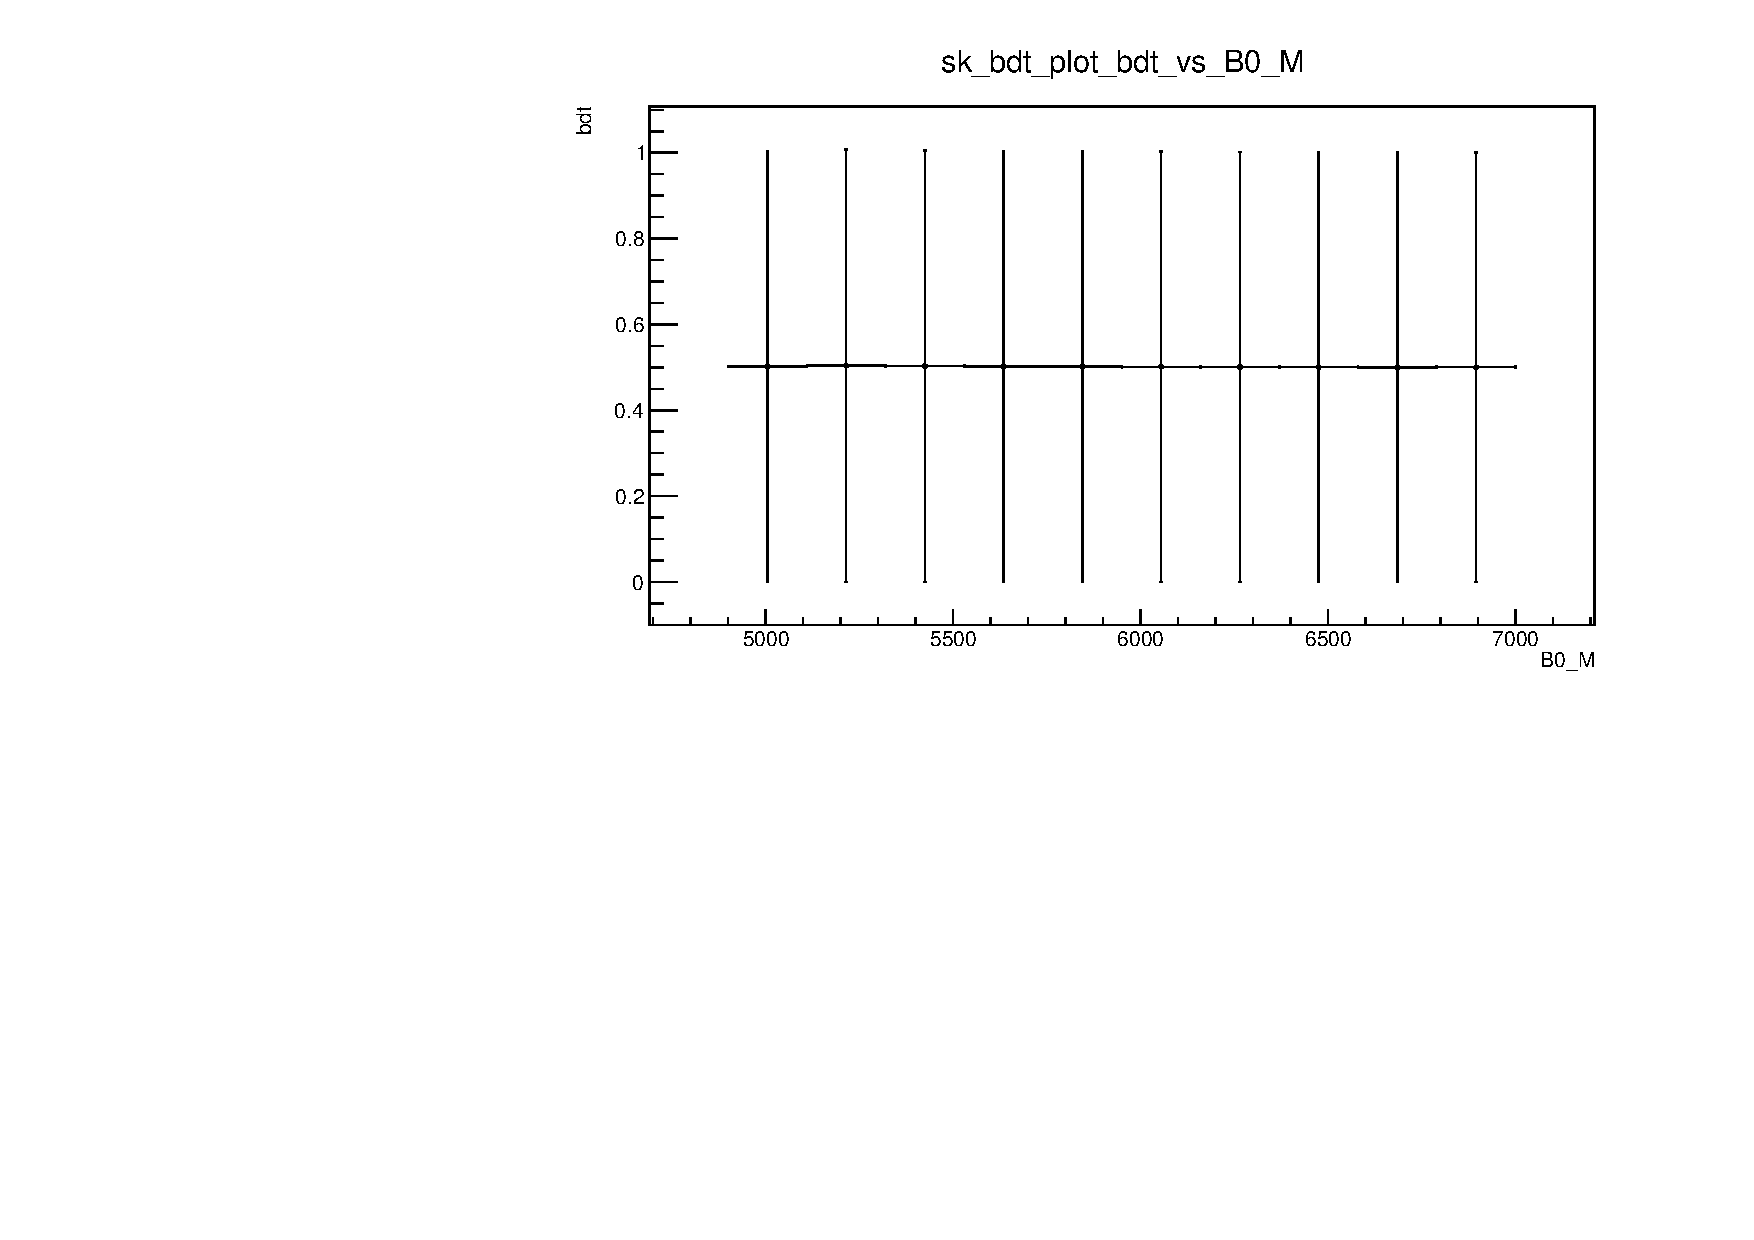
\includegraphics[width=0.5\textwidth]{plots/sk_bdt_plot_bdt_vs_B0_M}
  \caption{This plot shows the correlations between the probabilities to be signal assigned by the sk\_bdt classifier and the $B$ mass in MeV. There is no correlation.}
  \label{fig:skbdtB0M}
 \end{figure}

 \begin{figure}[H]
  \centering
  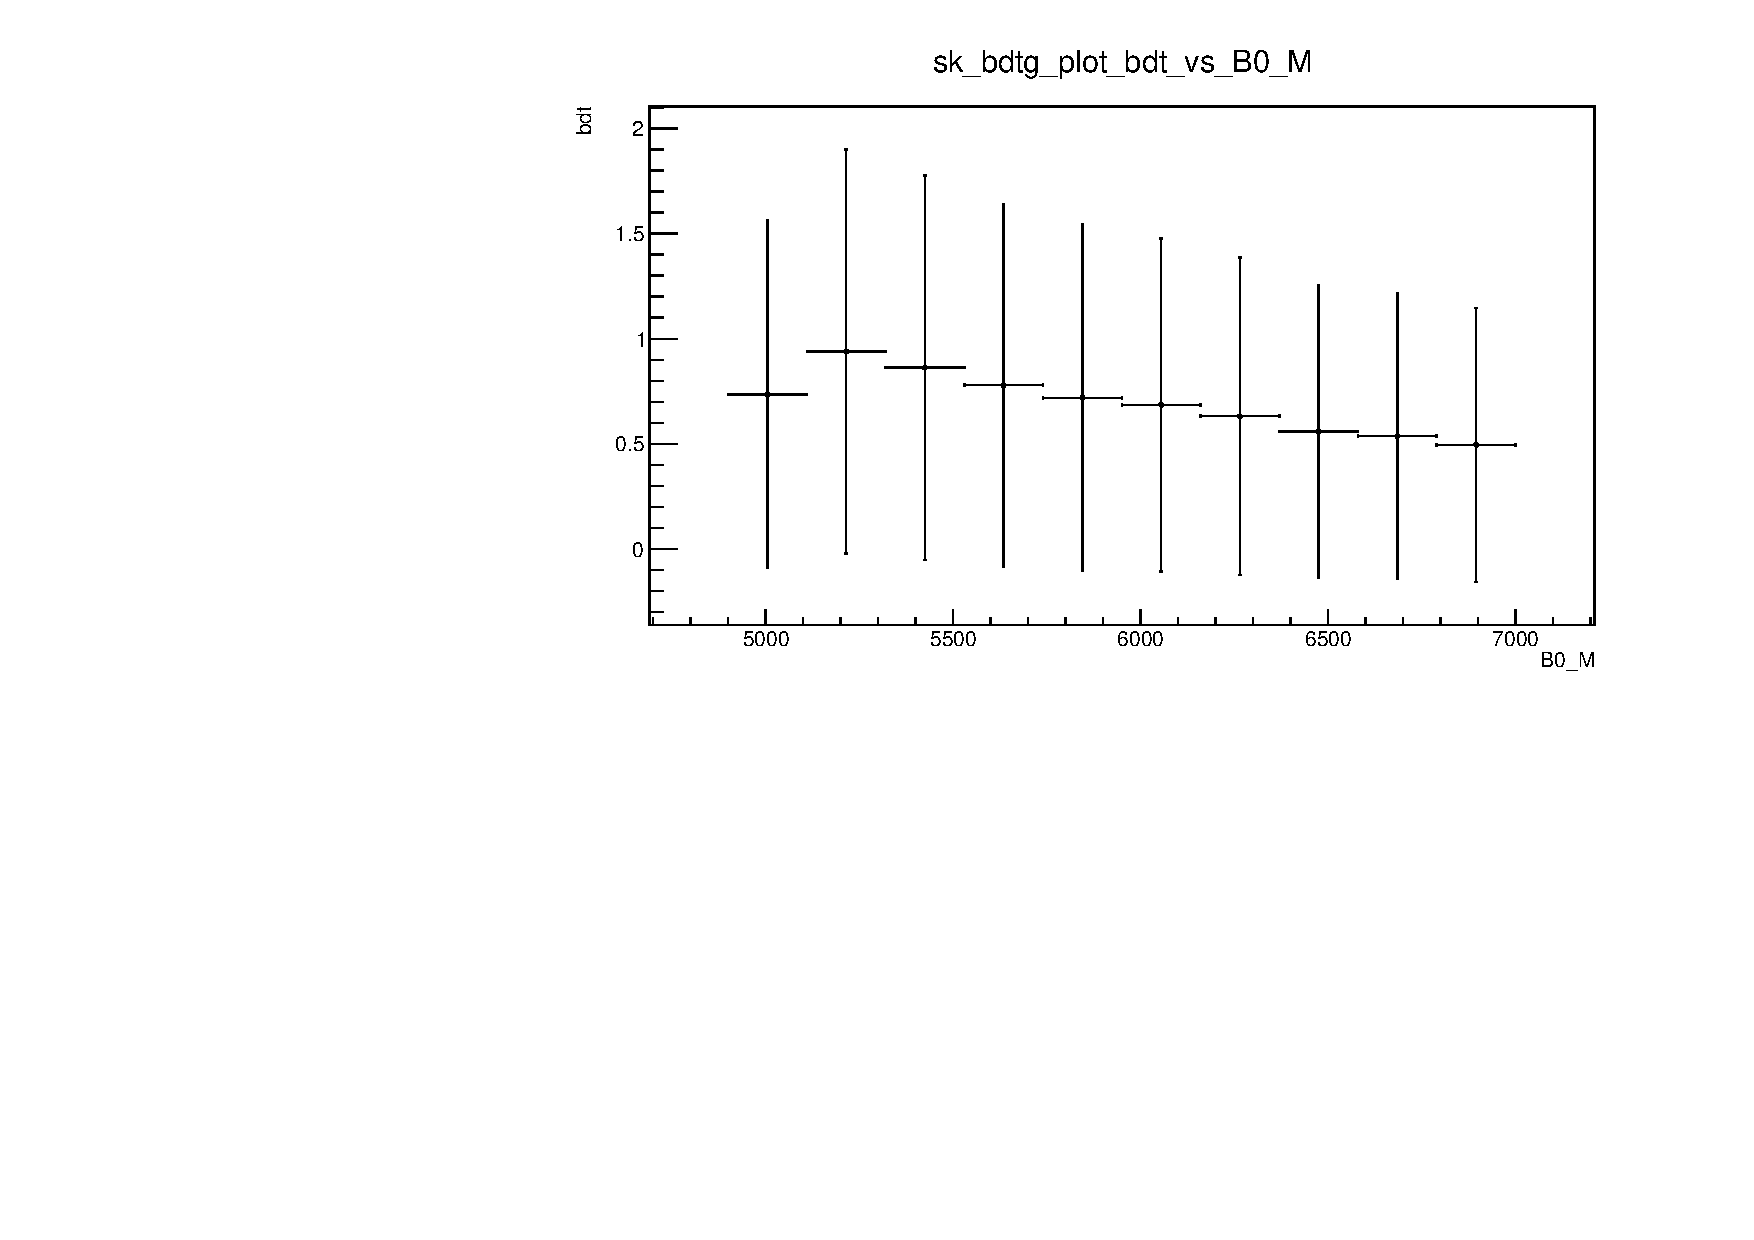
\includegraphics[width=0.5\textwidth]{plots/sk_bdtg_plot_bdt_vs_B0_M}
  \caption{This plot shows the correlations between the probabilities to be signal assigned by the sk\_bdtg classifier and the $B$ mass in MeV. There is a obvius correlation from the second bin to the fourth bin.}
  \label{fig:skbdtgB0M}
 \end{figure}

 \begin{figure}[H]
  \centering
  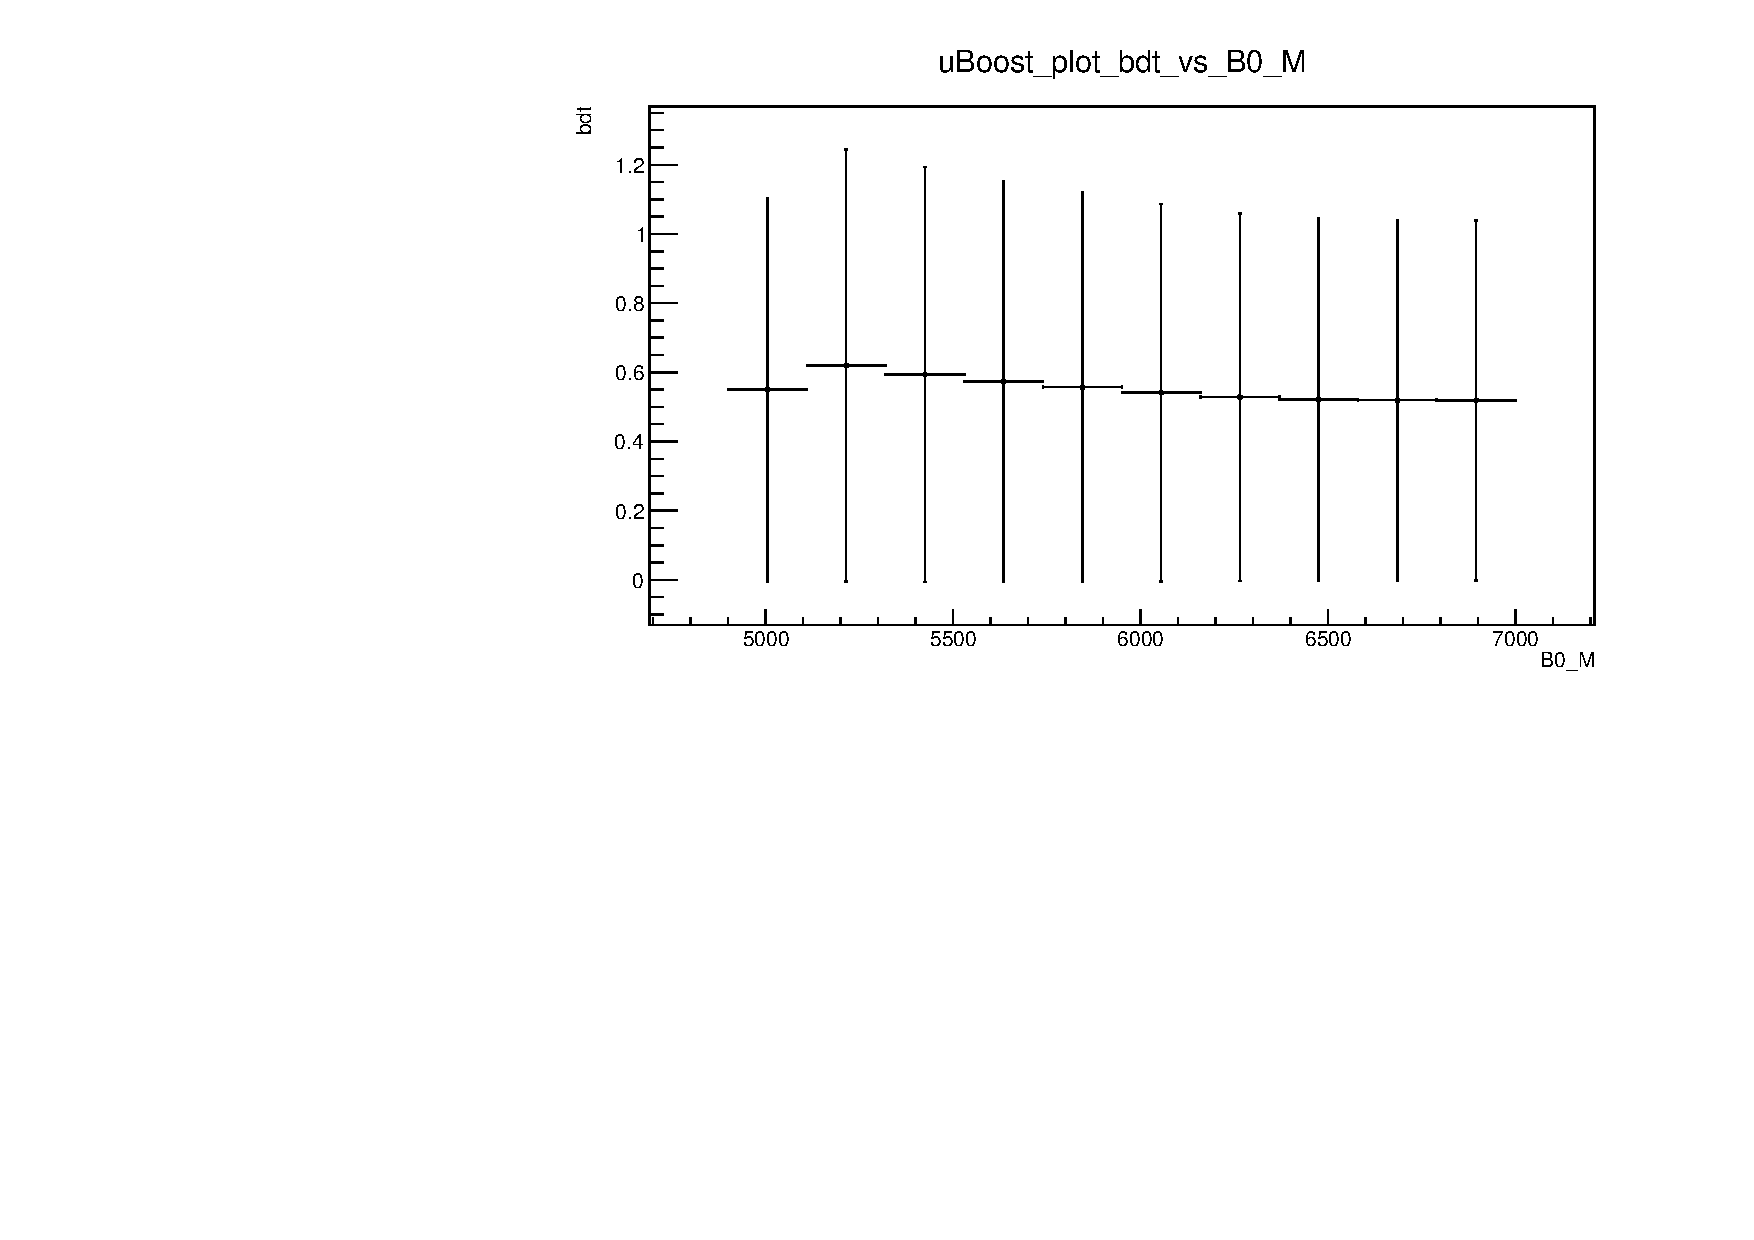
\includegraphics[width=0.5\textwidth]{plots/uBoost_plot_bdt_vs_B0_M}
  \caption{This plot shows the correlations between the probabilities to be signal assigned by the uBoost classifier and the $B$ mass in MeV. There is just a very small correlation compared to other classifiers.}
  \label{fig:uBoostB0M}
 \end{figure}

 \begin{figure}[H]
  \centering
  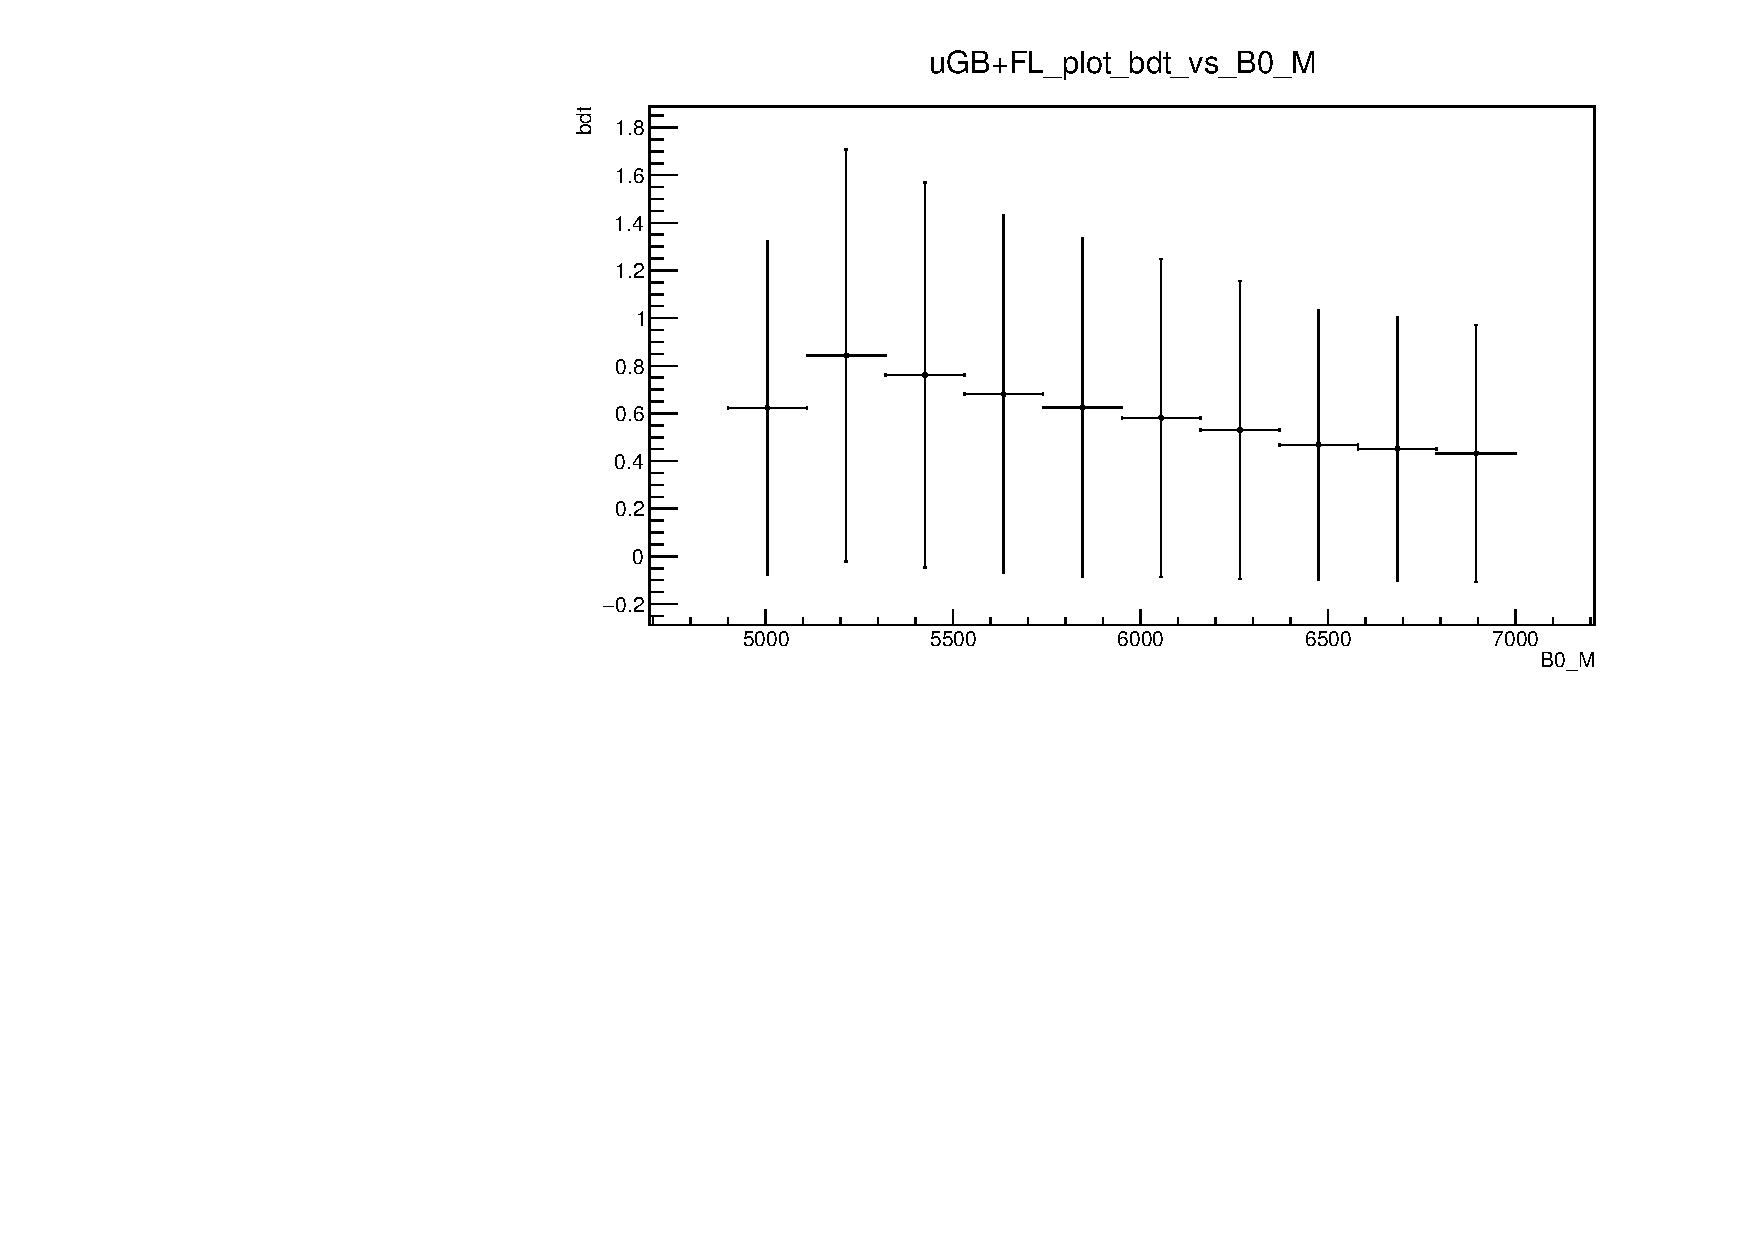
\includegraphics[width=0.5\textwidth]{plots/uGB+FL_plot_bdt_vs_B0_M}
  \caption{This plot shows the correlations between the probabilities to be signal assigned by the uGB+FL classifier and the $B$ mass in MeV. There is an obvius correlation from the second bin to the fourth bin.}
  \label{fig:uGB+FLB0M}
 \end{figure}

 \begin{figure}[H]
  \centering
  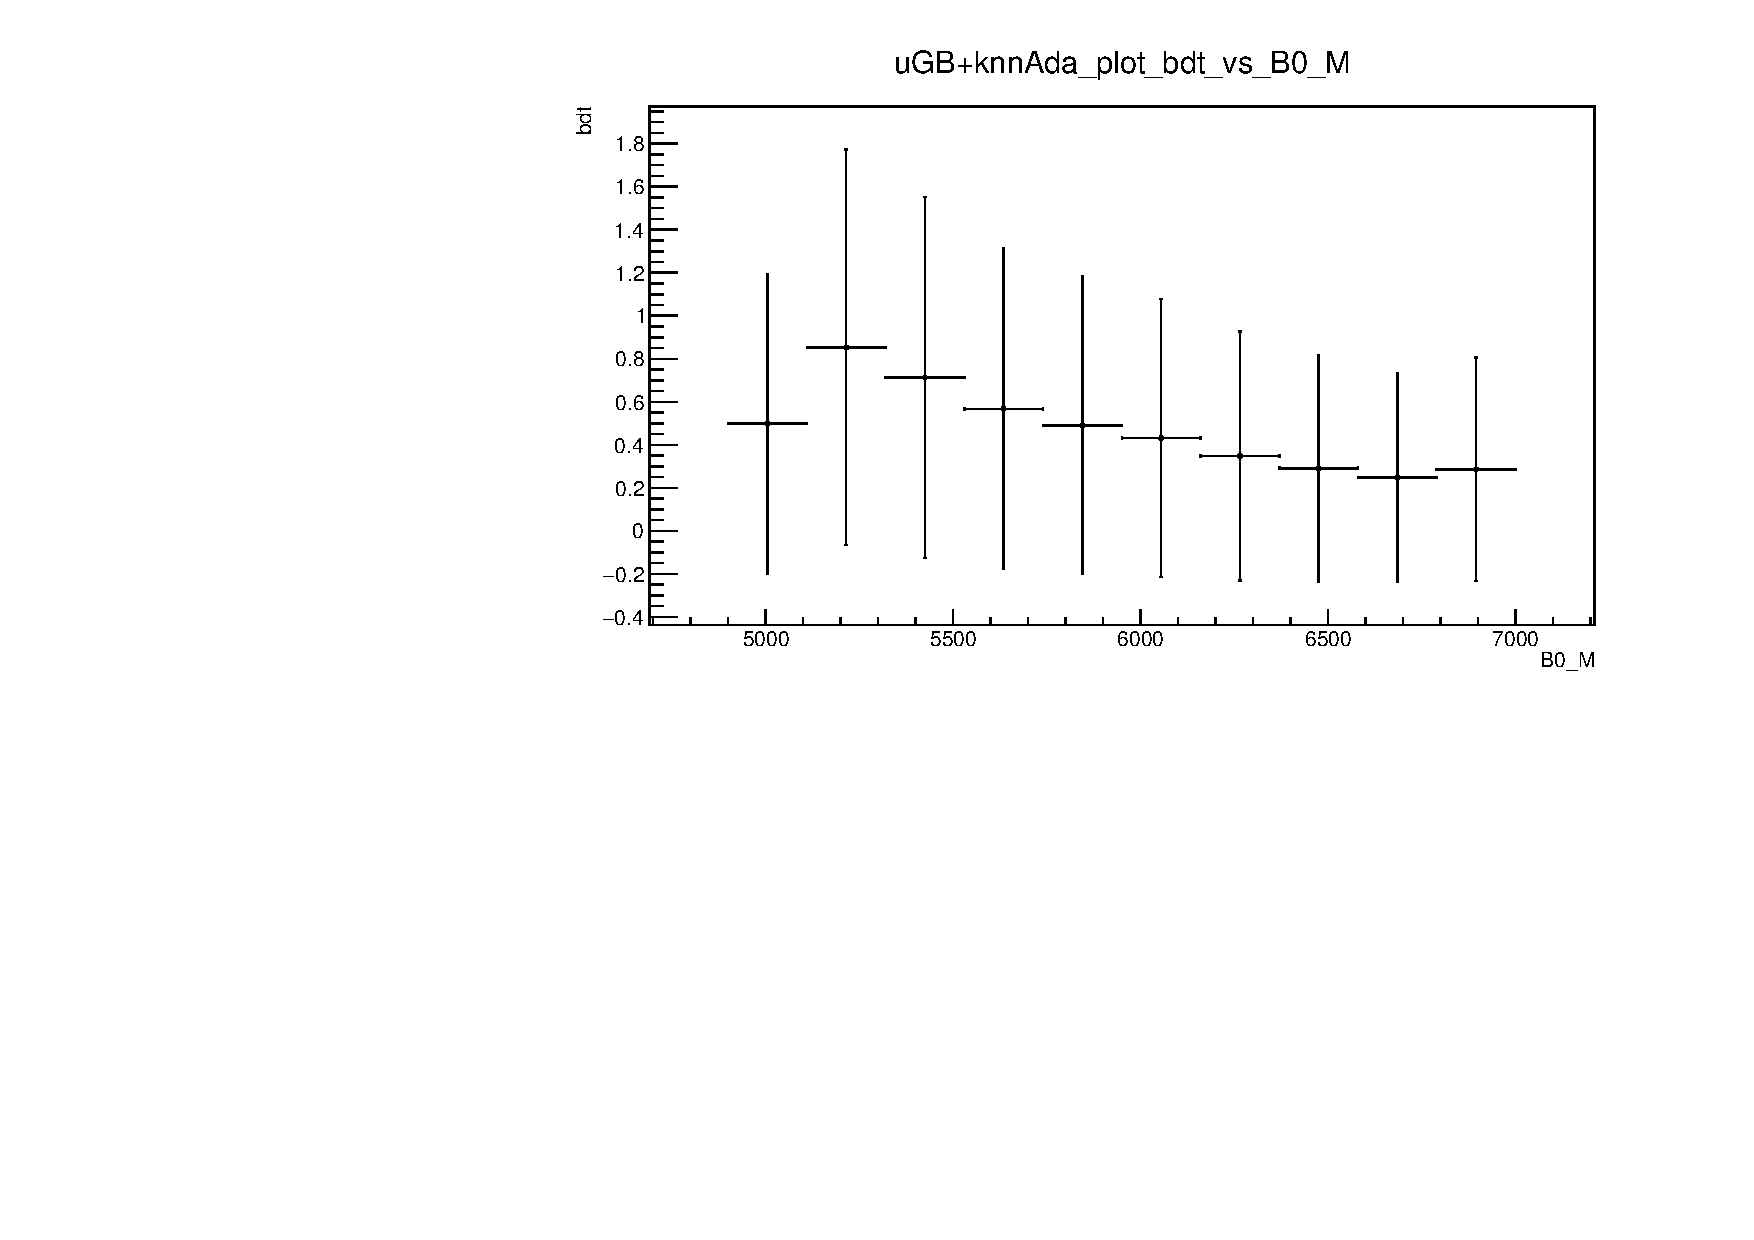
\includegraphics[width=0.5\textwidth]{plots/uGB+knnAda_plot_bdt_vs_B0_M}
  \caption{This plot shows the correlations between the probabilities to be signal assigned by the ugb+knnAda classifier and the $B$ mass in MeV. There is a obvius correlation from the second bin to the fourth bin.}
  \label{fig:uGB+knnAdaB0M}
 \end{figure}

 \begin{figure}[H]
  \centering
  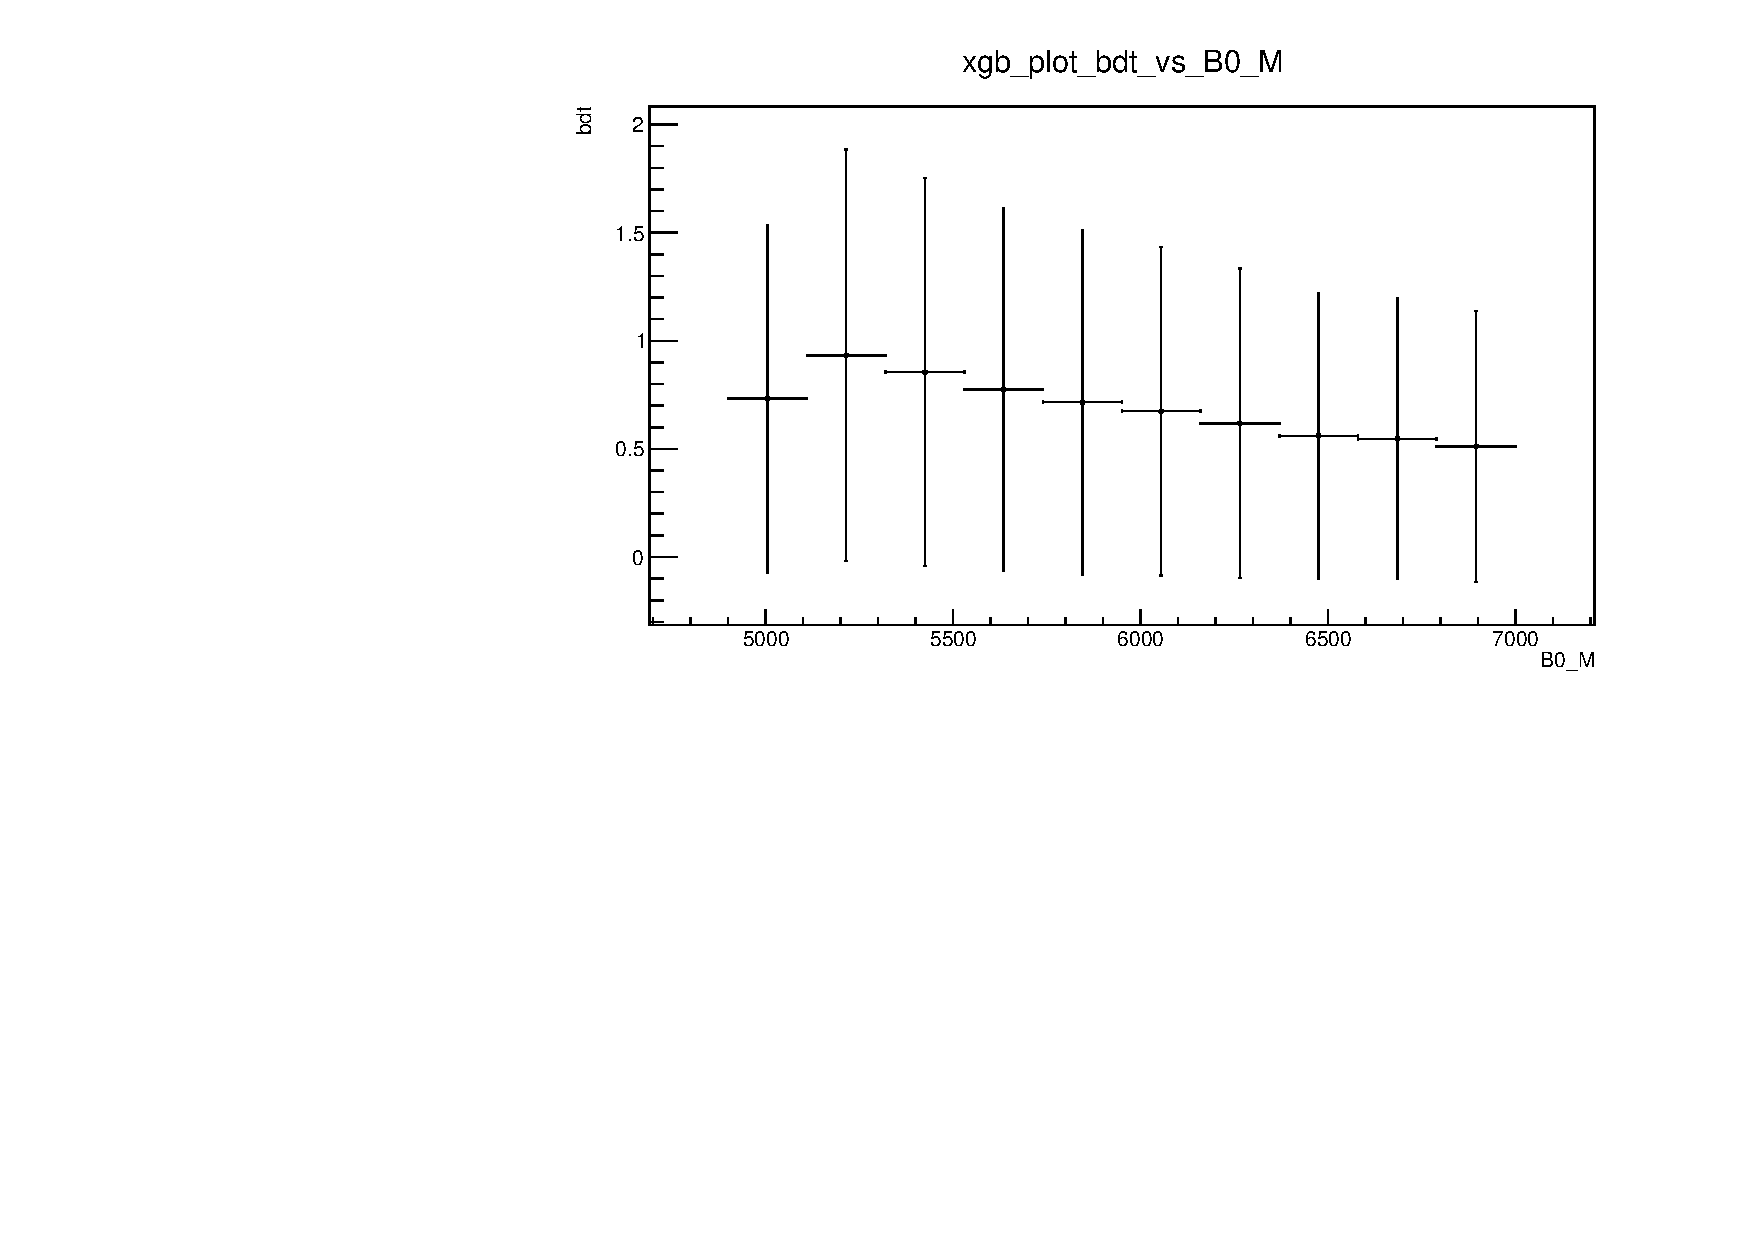
\includegraphics[width=0.5\textwidth]{plots/xgb_plot_bdt_vs_B0_M}
  \caption{This plot shows the correlations between the probabilities to be signal assigned by the xgb classifier and the $B$ mass in MeV. There is an obvius correlation from the second bin to the fourth bin.}
  \label{fig:xgbB0M}
 \end{figure}

 The two classifers with the least correlation are the sk\_bdt and the uBoost classifers. Therfore they could be used to do seperate between signal and background in the $B$ $\rightarrow$ $K^{*}$ $\mu$ $\mu$ data. But the uBoost classifer is a little bit better in the ROC curve (figure \ref{fig:roc}).



 \subsection{Reweighting} \label{sec:Reweight}

 % The infomation needed in an analysis is not all contained inside the data. For example efficiencies can not be recorded by a detector. But they can be simulated by a Monte Carlo simulation of the particle decay. The problem is that the simulation has to be the same as data to get the correct answers. Since resimulating everything with different parameters until one hits the data distribution would take too much resources. One can simply reweight the simulation to match the data.

Reweighting is a method to match the Monte Carlo data to the real detector data, to extract quantities not measurable by the detector itself like efficiencies. The match is done by applying weights to the Monte Carlo events. \\
As an initial weight the sWeights see equation \ref{eq:sWeight} are used. The parameters used for reweighting are applied in the following order:
\begin{itemize}
  \item number of tracks: 'nTracks'
  \item transversal momentum of the $B$ Meson: '$B$ $p_T$'
  \item quality of the $K \pi \mu \mu$ vertex. 'B vertex $\chi^2$'
\end{itemize}
The new weights derived by the difference in data and simulation of these parameters for the very clean channel $K^* \rightarrow J/ \Psi K^{*}$ \cite{bib:JPsi}, are used to reweight the $B \rightarrow K^* \mu \mu$ Monte Carlo sample.

\subsubsection{Results of the $B$ $\rightarrow$ $K^{*}$ $\mu$ $\mu$ reweighting}

\begin{figure}[H]
\centering
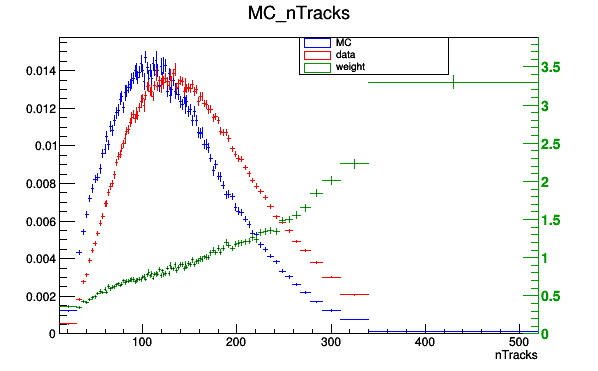
\includegraphics[width=0.8\textwidth]{Reweighting/nTracksw}
\caption{This plot shows the Monte Carlo Simulated data in blue, the detector data in red and in green the best weights to reweight the Monte Carlo data in order to match the detector data. The x- axes are the values for the number of tracks in an event (nTracks). On the left y-axes the fraction of events having nTracks is plotted. On the right y-axes the magnitude of the weights is shown.}
\label{fig:nTracksw}
\end{figure}

\begin{figure}[H]
\centering
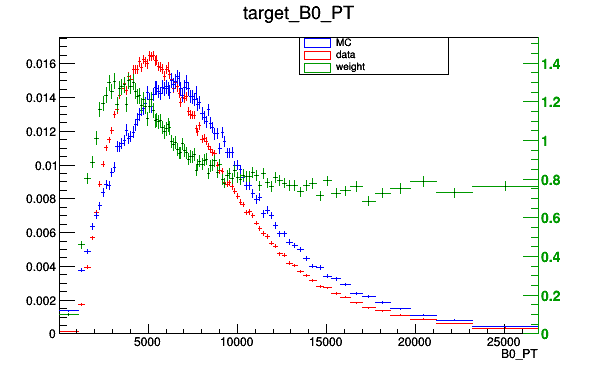
\includegraphics[width=0.8\textwidth]{Reweighting/B0_PTw}
\caption{Same plot as in figure \ref{fig:nTracksw}, for the transversal momentum of the $B$ meson (B0\_PT) in MeV.}
\label{fig:B0_PTw}
\end{figure}

\begin{figure}[H]
\centering
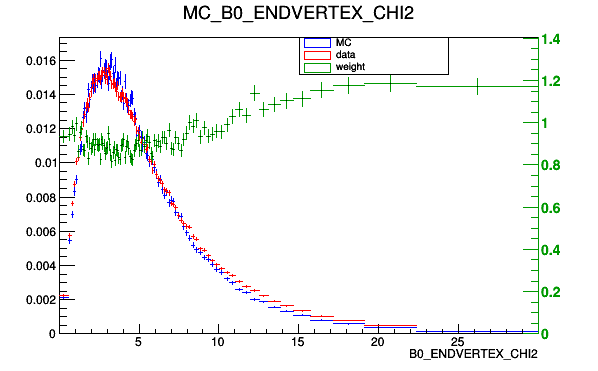
\includegraphics[width=0.8\textwidth]{Reweighting/B0_ENDVERTEX_CHI2w}
\caption{Same plot as in figure \ref{fig:nTracksw}, for the quality of the $K \pi \mu \mu$ vertex (B0\_ENDVERTEX\_CHI2).}
\label{fig:B0_ENDVERTEX_CHI2w}
\end{figure}

After applying those weights to the Monte Carlo data, the distributions of all the event parameters will change. To check if the simulation really matches the data. Some comparison plots have been made. One is presented here, while many others can be found in appendix \ref{app:re}.

\begin{figure}[H]
\centering
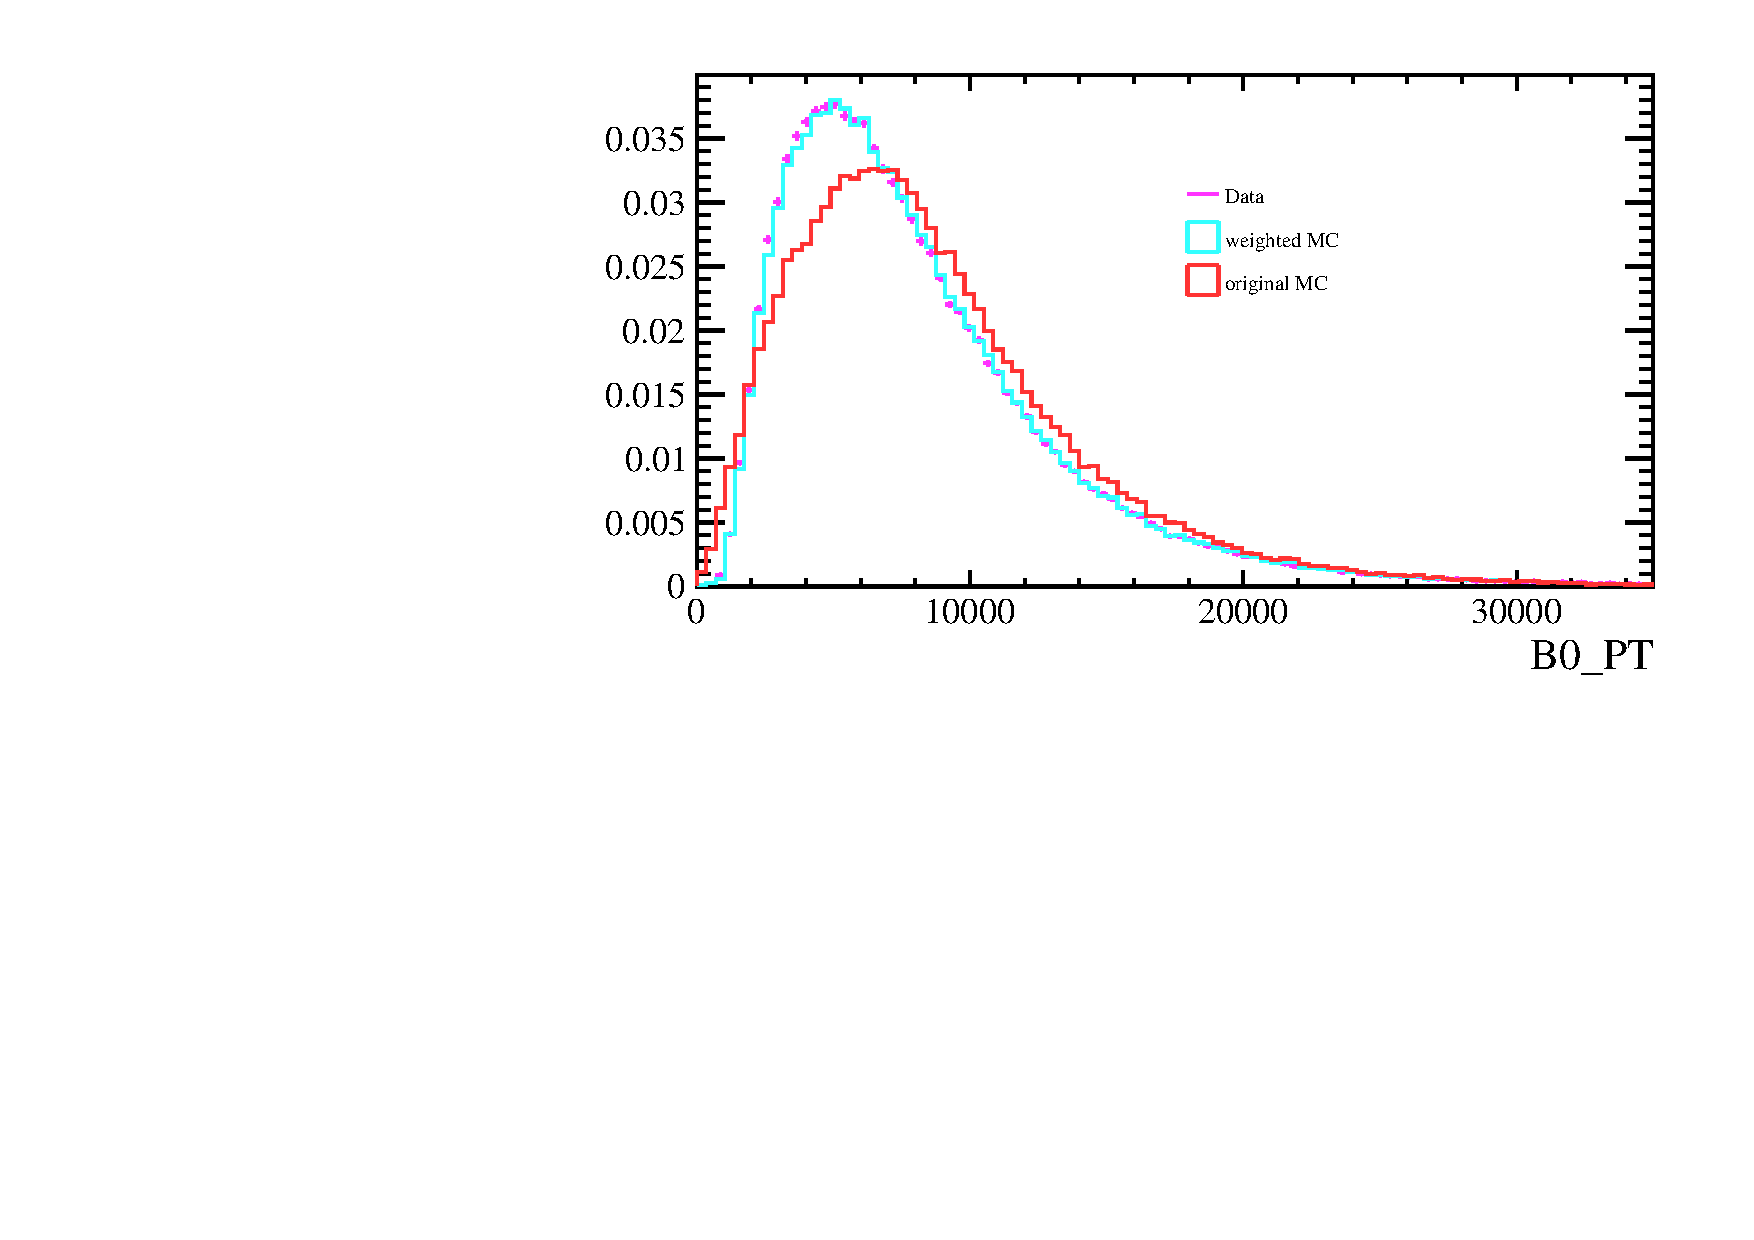
\includegraphics[width=0.8\textwidth]{Reweighting/B0_PT}
\caption{This plots shows the distribution of the $B$ transversal momentum. The X achsis shows the $B$ transversal momentum (B0\_PT) in MeV. The violet points represent the distribution of (B0\_PT) in the detector data.
The red line represents the distribution of (B0\_PT) before reweighting the Monte Carlo data.
The blue line represents the distribution (B0\_PT) after reweighting the Monte Carlo data. }
\label{fig:B0_PT}
\end{figure}




 \subsubsection{SPlot}
In this section the SPlot Technique is explained. It is used to separate two or more merged distributions and  has been used to get the initial weights for the re-weighting in this chapter.

 \subsubsection*{Likelihood method}
 Consider an analysis of a data sample, which consists of several types of events. These types represent signal components and background components, for example from different experiments. The log-liklihood of such a data sample is expressed as:
 \begin{align}
  L = \sum_{i=1}^{N} \ln \left[ \sum_{j=1}^{N_S} N_j f_j (y_i) \right] - \sum_{i=j}^{N_S} N_j \label{eq:L}
 \end{align}

 \begin{itemize}
  \item $N$ = total number of events \\
  \item $N_S$ = number of types \\
  \item $N_i$ = expected average number of events for type $i$ \\
  \item $y$ = set of diciminating variables \\
  \item $f_j$ = PDF of the $i$th type \\
  \item $f_j(y_i)$ = value of PDF for event $y_i$ \\
  \item $x$ = control variable, not a part of $L$ by construction
 \end{itemize}
 The yields $N_i$ and the free parameters of the PDF are obtained by maximizing the above log-likelihood (eq \ref{eq:L}).

 \subsubsection*{$_{in} Plot$ technique}
Consider a variable x which can be expressed as a function of the discriminating variables y used in the fit. Furthermore a fit has been performed to determine the yields $N_i$ for all types. From the knowledge of the PDF and the values of Ni a naive weight can be defined as:
 \begin{align}
  P_n(y_i) = \frac{N_n f_n(y_i)}{\sum_{k=1}^{N_s} N_k f_k(y_i)} \label{eq:P_n}
 \end{align}
which leads the the x-distribution $\tilde{M}_n$ defined by:
 \begin{align}
  N_n \tilde{M}_n (\bar{x}) = \sum_{i \subset \delta x} P_n (y_i) \label{eq:Mn}
 \end{align}
 where sum $\sum_{i \subset \delta x}$ contains alle events for which $x_i$ lies in the interval centered on $\bar{x}$ and of total width $\delta x$.
 Therefore $N_n \tilde{M}_n (\bar{x}) \delta x$ is the x-distribution of the histogrammed events, using the weights of eq \ref{eq:P_n}.
 With this procedure one can on average reproduce the true distribution $\textbf{M}_n(x)$. One can even replace the sum in eq \ref{eq:Mn} by an integral:
 \begin{align}
  \left \langle \sum_{i \subset \delta x} \right \rangle \rightarrow \int dy \sum_{j=1}^{N_s} N_j f_j (y) \delta (x(y) - \bar{x}) \delta x \label{eq:average}
 \end{align}
 Furthermore through identifying the number of events $N_i$ from the fit one gets:
 \begin{align}
  \langle N_n \rangle \tilde{M}_n (\bar{x}) & = \int dy \sum_{j=1}^{N_s} N_j f_j (y) \delta (x(y) - \bar{x}) P_n (y)                                               \\
                                            & = \int dy \sum_{j=1}^{N_s} N_j f_j (y) \delta (x(y)- \bar{x}) \cdot \frac{N_n f_n (y)}{\sum_{k=1}^{N_s} N_k f_k (y)} \\
                                            & = N_n \int dy \delta (x(y) - \bar{x}) f_n (y)                                                                        \\
                                            & = N_n \textbf{M}_n(\bar{x}) \label{eq:N_nM_n}
 \end{align}
 One can see that the sum over events of the naive weight $P_n$ provides a direct estimate of the x-distribution for the nth type.
 But this procedure has a major drawback. Since x is correlated to y, the PDFs of x enter implicity in the definition of the naive weight. Therefore the $\tilde{M}_n$ distributions are a bad estimate for the quality of the fit. These distributions are biased in a difficult way, when the PDFs $f_i(y)$ are not accurate. \\
 Consider for example a data sample where one of the types has events on the tail of the x-distribution. Such events require the true distribution to account for the tail. But since the events are averaged the weights on the tail are going to be very small missing those events in the estimated true distribution.
 Only the core of the x-distribution can be examined with $_{in} Plots$.


 \subsubsection*{$_{S} Plot$ technique}
 In the previous section it was shown that if a variable x belongs to a set y of discriminating varibales, the expected x distribution can be reconstruct.
 Consider now two sets of variables $x$ and $y$, where x does not belong to y and which are uncorrelated , hence the total PDFs $f_i (x,y)$ all factorize into products $\textbf{M}_i (x) f_i(y)$.
 The equation \ref{eq:N_nM_n} does not hold anymore because, when summing over the events the x-PDFs $\textbf{M}_j(x)$ appears:

 \begin{align}
  \langle N_n \rangle \tilde{M}_n (\bar{x}) & = \int \int dy dx \sum_{j=1}^{N_s} N_j \textbf{M}_j (x) f_j (y) \delta (x- \bar{x}) P_n \label{eq:M_nX}                    \\
                                            & = \int dy \sum_{j=1}^{N_s} N_j \textbf{M}_j (\bar{x}) f_j(y) \frac{N_n f_n(y)}{\sum_{k=1}^{N_s} N_k f_k(y)}                \\
                                            & = N_n \sum_{j=1}^{N_s} \textbf{M}_j (\bar{x}) \left( N_j \int dy \frac{f_n(y) f_j(y)}{\sum_{k=1}^{Ns} N_k f_k (y)} \right) \\
                                            & \neq N_n \textbf{M}_n (\bar{x}).
 \end{align}

 The correction term

 \begin{align}
  N_j \int dy \frac{f_n (y) f_j (y)}{\sum_{k=1}^{N_s} N_k f_k(y)}
 \end{align}
 is not identical to the kroenecker delta $\delta_{jn}$. In fact the $N_n \tilde{M}_n$ distribution obtained by the naive weight is a linear combination of the true distribution $\textbf{M}_j$. \\
 To go forward one has to realize that the correction term is related to the inverse of the covariance matrix, given by the second derivatives of $-L$, after the minimization.
 \begin{align}
  \textbf{V}_{nj}^{-1} = \frac{\partial^2 (-L)}{\partial N_n \partial N_j} = \sum_{i=1}^{N} \frac{f_n(y_i) f_j(y_i)} {\left( \sum_{k=1}^{N_s} N_k f_k(y_i) \right)^2}
 \end{align}
 If one averages and is replacing the sum over events by intergals (eq \ref{eq:average}) the varaince matrix reads:
 \begin{align}
  \langle \textbf{V}_{nj}^{-1} \rangle & = \int \int dy dx \sum_{e=1}^{N_s} N_e \textbf{M}_e(x) f_e(y) \frac{f_n(y) f_j(y)}{ \left( \sum_{k=1}^{N_s} N_k f_k(y) \right)^2}       \\
                                       & = \int dy \sum_{e=1}^{N_s} N_e f_e(y) \frac{f_n(y) f_j(y)}{ \left( \sum_{k=1}^{N_s} N_k f_k(y) \right)^2} \cdot \int dx \textbf{M}_l(x) \\
                                       & = \int dy \frac{f_n (y) f_j (y)}{\sum_{k=1}^{N_s} N_k f_k(y)}
 \end{align}
 Therefor equation \ref{eq:M_nX} can be rewritten as:
 \begin{align}
  \langle \tilde{M}_n (\bar{x}) \rangle = \sum_{j=1}^{N_s} \textbf{M}_j (\bar{x}) N_j \langle \textbf{V}_{nj}^{-1} \rangle .
 \end{align}
 To get the distribution of intrest one has to invert this matrix equation:
 \begin{align}
  N_n \textbf{M}_n(\bar{x}) = \sum_{j=1}^{N_s} \langle \textbf{V}_nj \rangle \langle \tilde{M}_j (\bar{x}) \rangle
 \end{align}
 The true distribution of $x$ can still be reconstructed using the naive weight (eq \ref{eq:P_n}), through a linear combination of $_{in} Plots$. In other words: When x does not belong to the set y, the weights are not given by equation \ref{eq:P_n}, they are given by a covariance-weighted quantity called sWeight defined by:
 \begin{align}
  _s P_n(y_i) = \frac{\sum_{j=1}^{N_s} \textbf{V}_nj f_j(y_i)} {\sum_{k=1}^{N_s} N_k f_k (y_i)} \label{eq:sWeight}
 \end{align}
 With the sWeights on can obtain the distribution of the x variable by histogramming the $_s Plot$:
 \begin{align}
  N_n { }_{s} \tilde{M}_n (\bar{x}) \delta x = \sum_{i \subset \delta x} { }_{s} P_n (y_i) \label{eq:sPlot2}
 \end{align}
 On average it reproduced the true distribution:
 \begin{align}
  \langle N_n { }_s \tilde{M}_n (x) \rangle = N_n \textbf{M}_n (x)
 \end{align}
In the case were x is significantly correlated with y, the sPlots from equation \ref{eq:sPlot2} can not be compared with the pure distributions of the various types. To solve that problem one can perform a Monte Carlo simulation of the procedure and obtain the expected distributions to which the $_s Plots$ should be compared. \\
More information on $_s Plots$ is given in reference \cite{bib:sPlot}.

\section{Summary}
The RooMCMarkovChain fitting routine is currently beeing added \cite{bib:pull} to the ROOT Data analysis framework. The best classifier uBoost from the classifers test will be used to find future $B \rightarrow K^* \mu \mu$ decays in the data produced by the LHCb detector. The rewighting done in this thesis will be used for the future analysis of the $B \rightarrow K^* \mu \mu$ in the current LHCb data.
%more physics

 \begin{thebibliography}{100}
   \addcontentsline{toc}{section}{Bibliography}

   \bibitem{bib:Likelihood} Likelihood Fits, Craig Blocker, Brandeis, 23.8.2004,
   \url{http://physics.bu.edu/neppsr/2004/Talks/Likelihood-Blocker.pdf}

    \bibitem{bib:MinuitRM} Minuit Reference Manual Version 94.1, \url{https://root.cern.ch/sites/d35c7d8c.web.cern.ch/files/minuit.pdf}

   \bibitem{bib:root} ROOT Data Analysis Framework \url{https://root.cern.ch/}

   \bibitem{bib:Minuit} MINUIT Home page, \url{https://seal.web.cern.ch/seal/snapshot/work-packages/mathlibs/minuit/}

   \bibitem{bib:LU} JHEP08 (2017) 055

   \bibitem{bib:Operators}  C. Bobeth, M. Misiak and J. Urban, Nucl. Phys. B 574 (2000) 291 [arXiv:hep-ph/9910220].

   \bibitem{bib:Wilson} 	arXiv:0811.1214 [hep-ph]

   \bibitem{bib:lhc_img} CERN Accelerator Complex,
   \url{http://www.stfc.ac.uk/research/particle-physics-and-particle-astrophysics/large-hadron-collider/cern-accelerator-complex/}

   \bibitem{bib:lhcb_detector} Science and Technology Facilities Council article about LHCb ,
   \url{https://www.ppd.stfc.ac.uk/Pages/LHCb.aspx}

   \bibitem{bib:velo} VELO description,
   \url{http://lhcb-public.web.cern.ch/lhcb-public/en/Detector/VELO2-en.html}

   \bibitem{bib:rich} RICH description,
   \url{http://lhcb-public.web.cern.ch/lhcb-public/en/Detector/RICH2-en.html}

   \bibitem{bib:mag} Magnet description,
   \url{http://lhcb-public.web.cern.ch/lhcb-public/en/Detector/Magnet2-en.html}

   \bibitem{bib:trac} Tracker description,
   \url{http://lhcb-public.web.cern.ch/lhcb-public/en/Detector/Trackers2-en.html}

   \bibitem{bib:calo} Calorimeters description,
   \url{http://lhcb-public.web.cern.ch/lhcb-public/en/Detector/Calorimeters2-en.html}

   \bibitem{bib:muonSys} Muon system description,
   \url{http://lhcb-public.web.cern.ch/lhcb-public/en/Detector/Muon2-en.html}

   \bibitem{bib:AdaBoost}  A Short Introduction to Boosting, by Yoav Freund and Rovert E. Schapire \url{http://www.site.uottawa.ca/~stan/csi5387/boost-tut-ppr.pdf}

   \bibitem{bib:ugb} J.H. Friedmann, " Greedy function approximation: A gradient boosting machine "  , 2001



   \bibitem{bib:uBoost}  J. Stevens and M. Williams, uBoost: A boosting method for producing uniform selection efficiencies from multivariate classifiers, JINST 8, P12013 (2013). [arXiv:1305.7248]

   \bibitem{bib:xgb}  arXiv:1603.02754 [cs.LG]

   \bibitem{bib:bdtg} Gradient Boosting classifier from the sk\_learn python package \url{http://scikit-learn.org/stable/modules/generated/sklearn.ensemble.GradientBoostingClassifier.html}

   \bibitem{bib:bdt} A vaiation of the AdaBoost classifier called AdaBoost-SAMME \url{http://scikit-learn.org/stable/modules/generated/sklearn.ensemble.AdaBoostClassifier.html}

   \bibitem{bib:JPsi} https://arxiv.org/pdf/1103.0423.pdf


   \bibitem{bib:sPlot} sPlot: a statistical tool to unfold data distributions,
   	arXiv:physics/0402083 [physics.data-an]

    \bibitem{bib:pull} https://github.com/root-project/root/pull/1422



 \end{thebibliography}

 \begin{appendix}
   \section{ROC curves}
   \label{app:roc}
   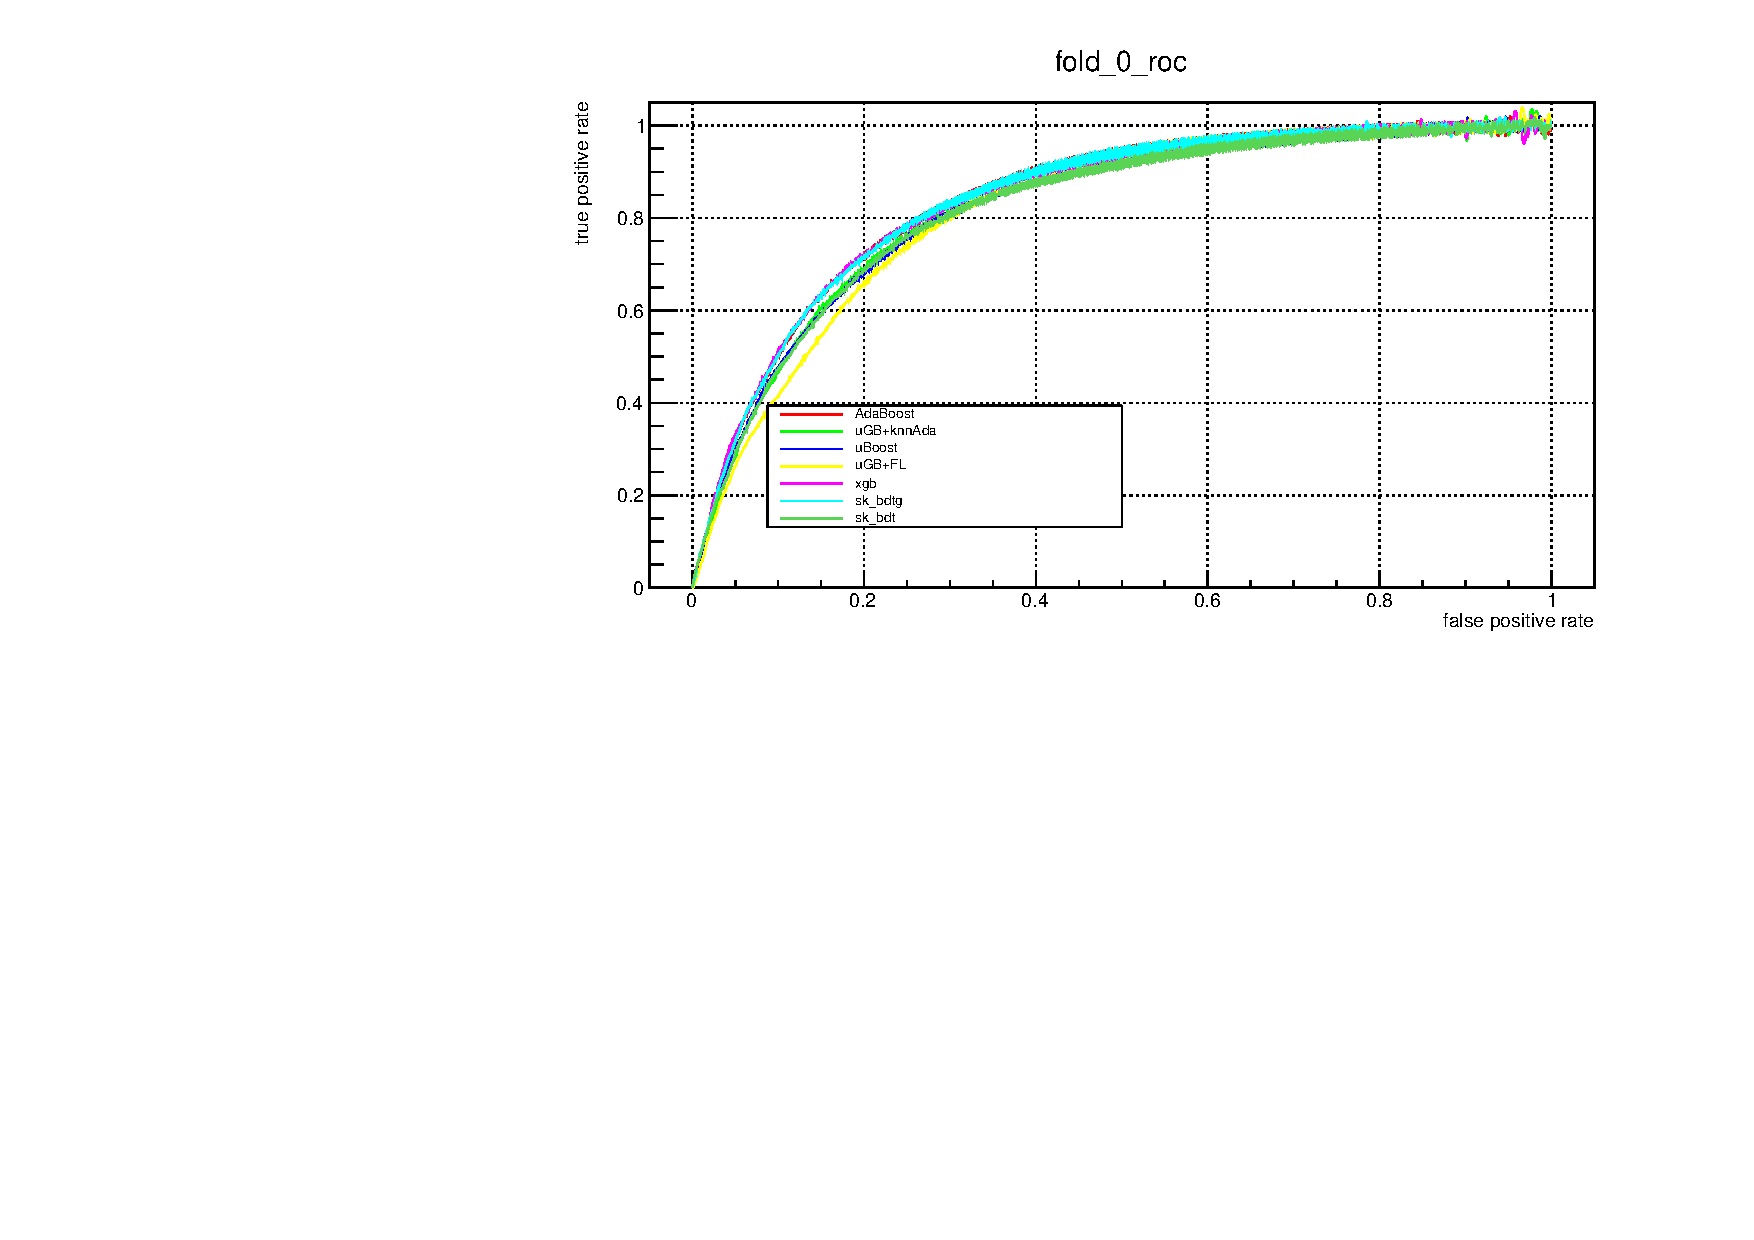
\includepdf[pages={-}]{roc.pdf}

   \section{Correlation plots}
   \label{app:corr}
   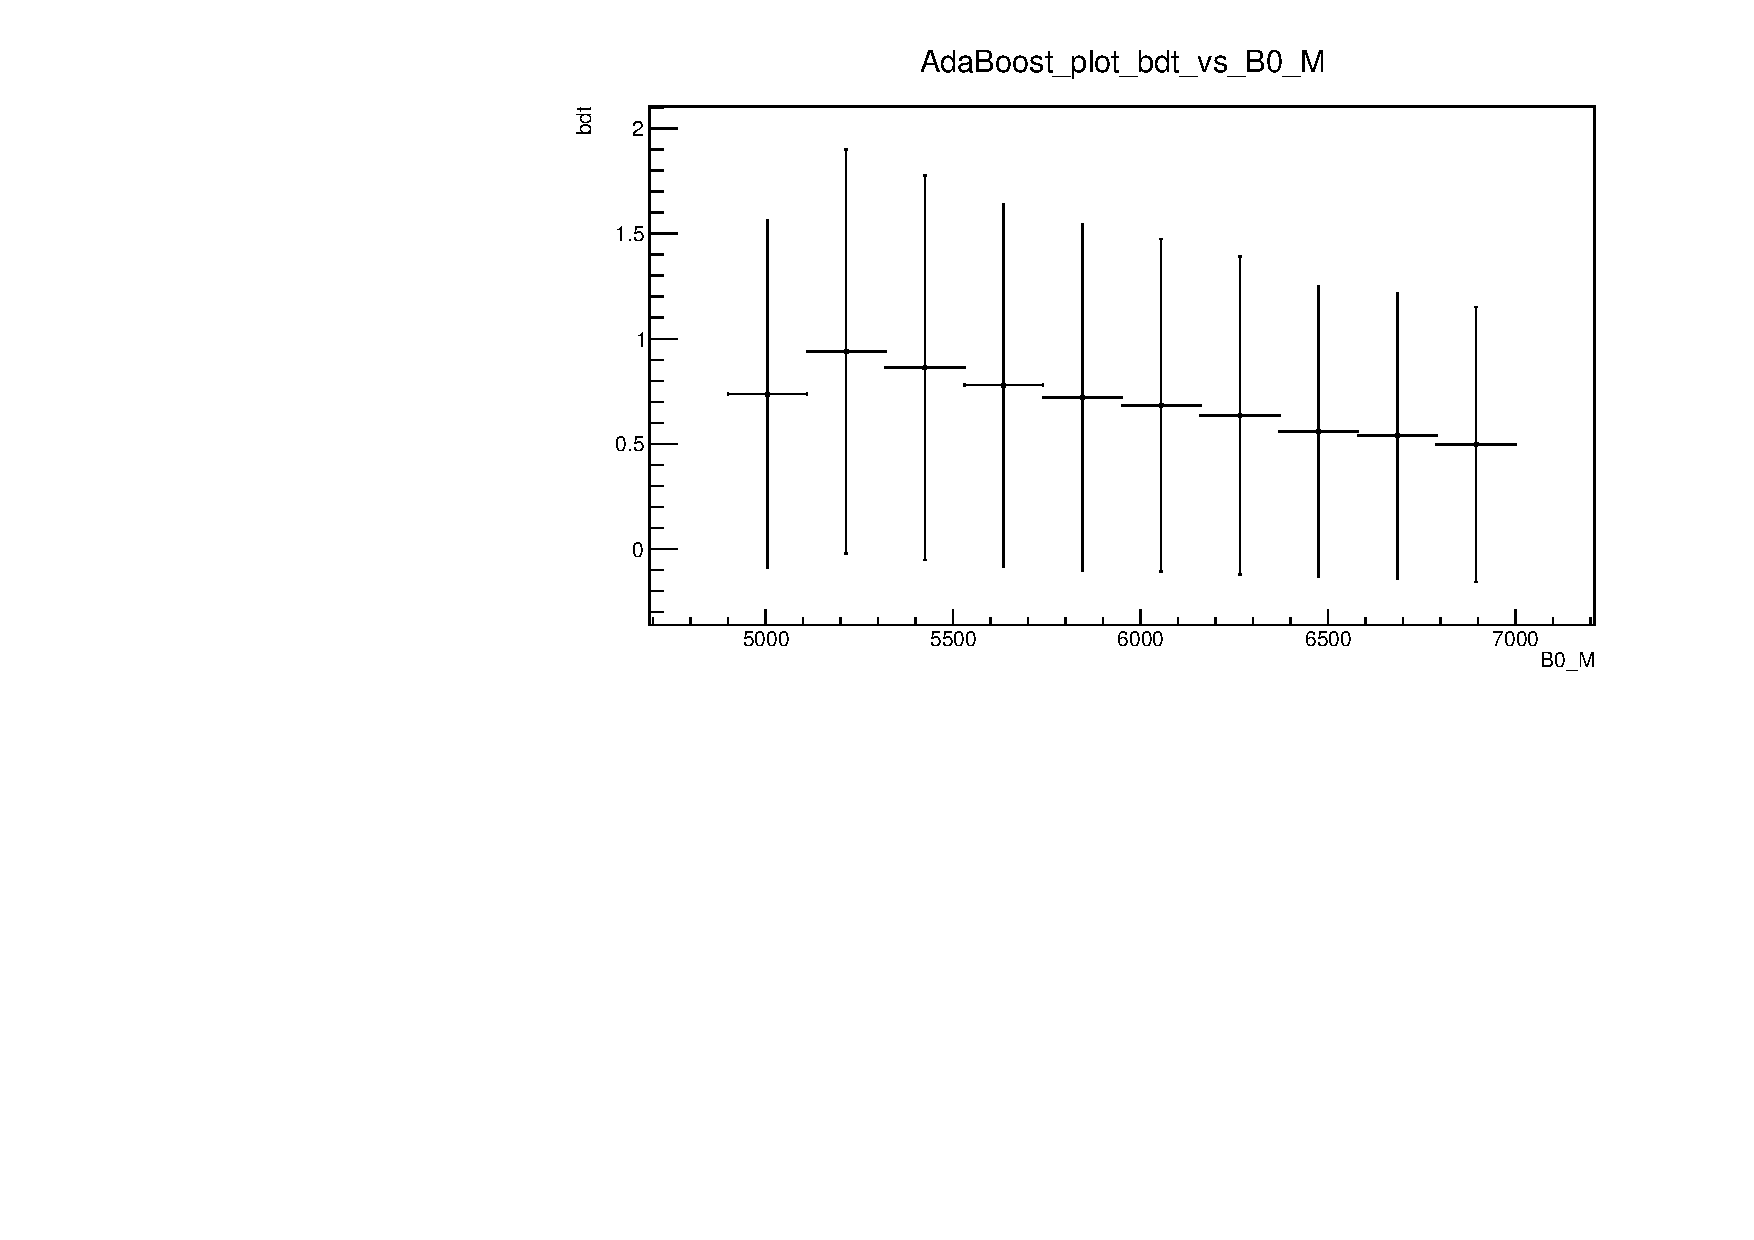
\includepdf[pages={-}]{Corplots.pdf}

   \section{Reweighting plots}
   \label{app:re}
   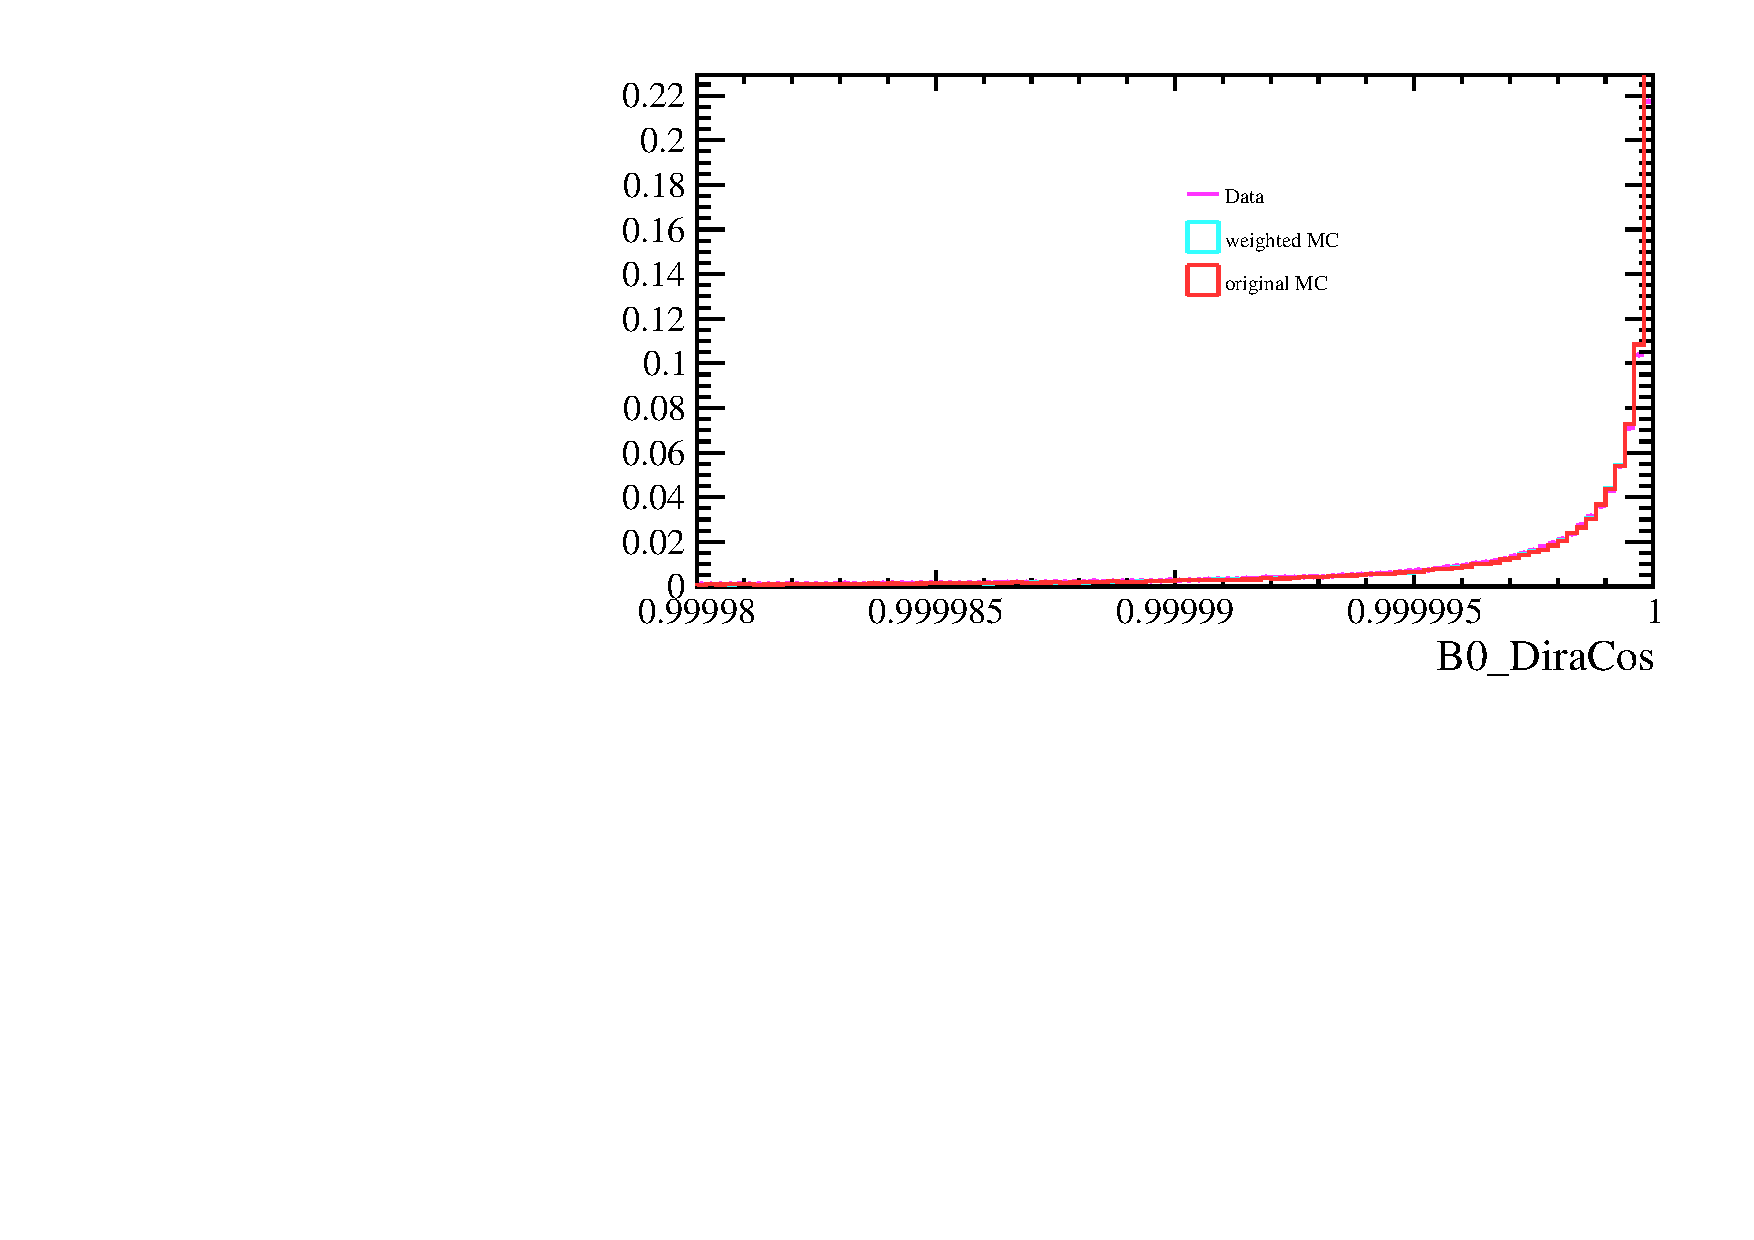
\includepdf[pages={-}]{Reweighting/reweight_app.pdf}

 \end{appendix}

 \end{document}
